% Specifica Tecnica
% da compilare con il comando pdflatex Specifica_tecnica_x.x.x.tex

% Dichiarazioni di ambiente e inclusione di pacchetti
% da usare tramite il comando % Dichiarazioni di ambiente e inclusione di pacchetti
% da usare tramite il comando % Dichiarazioni di ambiente e inclusione di pacchetti
% da usare tramite il comando \input{../../util/hx-ambiente}

\documentclass[a4paper,titlepage]{article}
\usepackage[T1]{fontenc}
\usepackage[utf8]{inputenc}
\usepackage[english,italian]{babel}
\usepackage{microtype}
\usepackage{lmodern}
\usepackage{underscore}
\usepackage{graphicx}
\usepackage{eurosym}
\usepackage{float}
\usepackage{fancyhdr}
\usepackage[table]{xcolor}
\usepackage{longtable}
\usepackage{chngpage}
\usepackage{grffile}
\usepackage[titles]{tocloft}
\usepackage{hyperref}
\hypersetup{hidelinks}

\usepackage{../../util/hx-vers}
\usepackage{../../util/hx-macro}
\usepackage{../../util/hx-front}

% solo se si vuole una nuova pagina ad ogni \section:
\usepackage{titlesec}
\newcommand{\sectionbreak}{\clearpage}

% stile di pagina:
\pagestyle{fancy}

% solo se si vuole eliminare l'indentazione ad ogni paragrafo:
\setlength{\parindent}{0pt}

% intestazione:
\lhead{\Large{\proj}}
\rhead{
\includegraphics[keepaspectratio=true,width=50px]{../../util/hivex_logo2.png}}
\renewcommand{\headrulewidth}{0.4pt}

% pie' di pagina:
\lfoot{\email}
\rfoot{\thepage}
\cfoot{}
\renewcommand{\footrulewidth}{0.4pt}

% spazio verticale tra le celle di una tabella:
\renewcommand{\arraystretch}{1.5}

% profondità di indicizzazione:
\setcounter{tocdepth}{4}
\setcounter{secnumdepth}{4}


\documentclass[a4paper,titlepage]{article}
\usepackage[T1]{fontenc}
\usepackage[utf8]{inputenc}
\usepackage[english,italian]{babel}
\usepackage{microtype}
\usepackage{lmodern}
\usepackage{underscore}
\usepackage{graphicx}
\usepackage{eurosym}
\usepackage{float}
\usepackage{fancyhdr}
\usepackage[table]{xcolor}
\usepackage{longtable}
\usepackage{chngpage}
\usepackage{grffile}
\usepackage[titles]{tocloft}
\usepackage{hyperref}
\hypersetup{hidelinks}

\usepackage{../../util/hx-vers}
\usepackage{../../util/hx-macro}
\usepackage{../../util/hx-front}

% solo se si vuole una nuova pagina ad ogni \section:
\usepackage{titlesec}
\newcommand{\sectionbreak}{\clearpage}

% stile di pagina:
\pagestyle{fancy}

% solo se si vuole eliminare l'indentazione ad ogni paragrafo:
\setlength{\parindent}{0pt}

% intestazione:
\lhead{\Large{\proj}}
\rhead{
\includegraphics[keepaspectratio=true,width=50px]{../../util/hivex_logo2.png}}
\renewcommand{\headrulewidth}{0.4pt}

% pie' di pagina:
\lfoot{\email}
\rfoot{\thepage}
\cfoot{}
\renewcommand{\footrulewidth}{0.4pt}

% spazio verticale tra le celle di una tabella:
\renewcommand{\arraystretch}{1.5}

% profondità di indicizzazione:
\setcounter{tocdepth}{4}
\setcounter{secnumdepth}{4}


\documentclass[a4paper,titlepage]{article}
\usepackage[T1]{fontenc}
\usepackage[utf8]{inputenc}
\usepackage[english,italian]{babel}
\usepackage{microtype}
\usepackage{lmodern}
\usepackage{underscore}
\usepackage{graphicx}
\usepackage{eurosym}
\usepackage{float}
\usepackage{fancyhdr}
\usepackage[table]{xcolor}
\usepackage{longtable}
\usepackage{chngpage}
\usepackage{grffile}
\usepackage[titles]{tocloft}
\usepackage{hyperref}
\hypersetup{hidelinks}

\usepackage{../../util/hx-vers}
\usepackage{../../util/hx-macro}
\usepackage{../../util/hx-front}

% solo se si vuole una nuova pagina ad ogni \section:
\usepackage{titlesec}
\newcommand{\sectionbreak}{\clearpage}

% stile di pagina:
\pagestyle{fancy}

% solo se si vuole eliminare l'indentazione ad ogni paragrafo:
\setlength{\parindent}{0pt}

% intestazione:
\lhead{\Large{\proj}}
\rhead{
\includegraphics[keepaspectratio=true,width=50px]{../../util/hivex_logo2.png}}
\renewcommand{\headrulewidth}{0.4pt}

% pie' di pagina:
\lfoot{\email}
\rfoot{\thepage}
\cfoot{}
\renewcommand{\footrulewidth}{0.4pt}

% spazio verticale tra le celle di una tabella:
\renewcommand{\arraystretch}{1.5}

% profondità di indicizzazione:
\setcounter{tocdepth}{4}
\setcounter{secnumdepth}{4}


\version{1.0.0}
\creaz{15 febbraio 2017}
\author{\ALL}
\supervisor{\MM}
\uso{esterno}
\dest{\ALL}
\title{Specifica Tecnica}
% \date{9 gennaio 2017}

% Per neutralizzare \nogloxy:
\newcommand{\nogloxy}[1]{#1}
\newcommand{\subsubsubsection}[1]{\paragraph{#1}}
\newcommand{\textt}[1]{\texttt{#1}}

% Elenco dei design pattern utilizzati in un documento:
\newcommand{\listpatternname}{Elenco dei \emph{design pattern}}
\newlistof{pattern}{pat}{\listpatternname}
\newcommand{\pattern}[1]{%
\refstepcounter{pattern}
\emph{#1}
\addcontentsline{pat}{pattern}{\protect\numberline{\thepattern}#1}}

\begin{document}
\maketitle
% diario delle modifiche per il piano di progetto
% da includere con % diario delle modifiche per il piano di progetto
% da includere con % diario delle modifiche per il piano di progetto
% da includere con \include{diario}

\begin{diario}
	1.0.1 & {\GG} (Responsabile) & 03/02/2017 & Correzione degli errori individuati nelle prime tre sezioni del documento \\ \hline
	1.0.0 & {\PB} (Responsabile) & 09/01/2017 & Approvazione documento \\ \hline
	0.1.0 & {\MM} (Verificatore) & 07/01/2017 & Verifica documento \\ \hline
	0.0.9 & {\PB} (Responsabile) & 05/01/2017 & Stesura Organigramma \\ \hline
	0.0.8 & {\LB} (Responsabile) & 05/01/2017 & Stesura Consuntivo di Periodo \\ \hline
	0.0.7 & {\LB} (Responsabile) & 04/01/2017 & Stesura Preventivo di Periodo \\ \hline
	0.0.6 & {\LB} (Responsabile) & 03/01/2017 & Inserimento Gantt Diagrammi delle Attività \\ \hline
	0.0.5 & {\PB} (Responsabile) & 29/12/2016 & Stesura Pianificazione delle Attività \\ \hline
	0.0.4 & {\PB} (Responsabile) & 28/12/2016 & Stesura Introduzione \\ \hline
	0.0.3 & {\LB} (Responsabile) & 27/12/2016 & Stesura Modello di sviluppo \\ \hline
	0.0.2 & {\PB} (Responsabile) & 27/12/2016 & Stesura Analisi dei Rischi \\ \hline
	0.0.1 & {\LB} (Responsabile) & 26/12/2016 & Stesura scheletro \\ \hline
\end{diario}

\begin{diario}
	1.0.1 & {\GG} (Responsabile) & 03/02/2017 & Correzione degli errori individuati nelle prime tre sezioni del documento \\ \hline
	1.0.0 & {\PB} (Responsabile) & 09/01/2017 & Approvazione documento \\ \hline
	0.1.0 & {\MM} (Verificatore) & 07/01/2017 & Verifica documento \\ \hline
	0.0.9 & {\PB} (Responsabile) & 05/01/2017 & Stesura Organigramma \\ \hline
	0.0.8 & {\LB} (Responsabile) & 05/01/2017 & Stesura Consuntivo di Periodo \\ \hline
	0.0.7 & {\LB} (Responsabile) & 04/01/2017 & Stesura Preventivo di Periodo \\ \hline
	0.0.6 & {\LB} (Responsabile) & 03/01/2017 & Inserimento Gantt Diagrammi delle Attività \\ \hline
	0.0.5 & {\PB} (Responsabile) & 29/12/2016 & Stesura Pianificazione delle Attività \\ \hline
	0.0.4 & {\PB} (Responsabile) & 28/12/2016 & Stesura Introduzione \\ \hline
	0.0.3 & {\LB} (Responsabile) & 27/12/2016 & Stesura Modello di sviluppo \\ \hline
	0.0.2 & {\PB} (Responsabile) & 27/12/2016 & Stesura Analisi dei Rischi \\ \hline
	0.0.1 & {\LB} (Responsabile) & 26/12/2016 & Stesura scheletro \\ \hline
\end{diario}

\begin{diario}
	1.0.1 & {\GG} (Responsabile) & 03/02/2017 & Correzione degli errori individuati nelle prime tre sezioni del documento \\ \hline
	1.0.0 & {\PB} (Responsabile) & 09/01/2017 & Approvazione documento \\ \hline
	0.1.0 & {\MM} (Verificatore) & 07/01/2017 & Verifica documento \\ \hline
	0.0.9 & {\PB} (Responsabile) & 05/01/2017 & Stesura Organigramma \\ \hline
	0.0.8 & {\LB} (Responsabile) & 05/01/2017 & Stesura Consuntivo di Periodo \\ \hline
	0.0.7 & {\LB} (Responsabile) & 04/01/2017 & Stesura Preventivo di Periodo \\ \hline
	0.0.6 & {\LB} (Responsabile) & 03/01/2017 & Inserimento Gantt Diagrammi delle Attività \\ \hline
	0.0.5 & {\PB} (Responsabile) & 29/12/2016 & Stesura Pianificazione delle Attività \\ \hline
	0.0.4 & {\PB} (Responsabile) & 28/12/2016 & Stesura Introduzione \\ \hline
	0.0.3 & {\LB} (Responsabile) & 27/12/2016 & Stesura Modello di sviluppo \\ \hline
	0.0.2 & {\PB} (Responsabile) & 27/12/2016 & Stesura Analisi dei Rischi \\ \hline
	0.0.1 & {\LB} (Responsabile) & 26/12/2016 & Stesura scheletro \\ \hline
\end{diario}
\tableofcontents
% \listofpattern



% - introduzione standard
% - stime di fattibilità
\section{Introduzione}
%%%%%%%%%%%%%%%%
%%  Introduzione
%%%%%%%%%%%%%%%%

\subsection{Scopo del documento}
Questo documento ha lo scopo di definire, ad alto livello, l'architettura software di \proj; ci focalizziamo quindi sulla \emph{struttura} del software, cioè sulla descrizione delle sue componenti. L'implementazione del nostro software è a oggetti; per questo, le componenti descritte sono classi e loro istanze.
% Ecco una prova di pattern: \pattern{Observer}

Riteniamo che l'architettura esposta di seguito, accompagnata da un documento più preciso che verrà prodotto nelle prossime settimane (Definizione di Prodotto), sia ragionevole e fattibile. La difficoltà di generare codice eseguibile è stata superata grazie ad un uso accorto di librerie open-source, stili architetturali e \emph{design patter}. Il tutto è stato svolto con grande attenzione ai princìpi della programmazione ad oggetti, per aumentare il grado di coesione di un'architettura che rischia ad ogni momento di gonfiarsi inutilmente.

Ci è parso utile indicizzare i \emph{design patter} utilizzati; per questo, li abbiamo riportati in un elenco (dopo l'indice generale).

\subsection{Scopo del prodotto}
\scopo

\subsection{Glossario}
\presgloss

\subsection{Riferimenti} \label{sec:ref}

\subsubsection{Riferimenti normativi}
% ...

\subsubsection{Riferimenti informativi}
\begin{itemize}
	\item E. Gamma, R. Helm, R. Johnson, J. Vlissides, \emph{Design Patterns: Elements of Reusable Object-Oriented Software}.
\end{itemize}


% - scelta di linguaggi, framework, librerie etc...
% - interfacce con tali tecnologie
\section{Tecnologie utilizzate}
%%%%%%%%%%%%%%%%%%%%%%%%%
%%  Tecnologie utilizzate
%%%%%%%%%%%%%%%%%%%%%%%%%



\subsection{\gloss{Client}}
Per implementare il client di \proj{} abbiamo scelto di utilizzare \gloss{HTML5} e \gloss{CSS3} assieme a \gloss{JavaScript}. Di seguito elenchiamo e descriviamo le librerie JavaScript di cui il nostro client necessita. Tutte le librerie sono open-source, come richiesto dal capitolato.

\subsubsection{JointJS}
La libreria \jointjs{} (\url{https://www.jointjs.com/opensource}) è una libreria open-source per realizzare \gloss{editor} di diagrammi interattivi, in maniera altamente personalizzabile. %Dipende da HTML5 e da alcune altre librerie JavaScript ma offre numerosi plug-in per realizzare particolari tipi di grafi.

La libreria sfrutta le seguenti tecnologie per il suo funzionamento:

\begin{itemize}
	\item \\gloss{html}{}: \jointjs{} richiede che una pagina \html{} sia popolata con un tag \texttt{<svg>}, che conterrà un diagramma.
	\item Le seguenti librerie \js{}:
	\begin{itemize}
		\item \jquery{};
		\item \lodash{};
		\item \backbonejs{}.
	\end{itemize}
\end{itemize}

\subsubsection{\backbonejs}
La libreria \backbonejs{} permette di strutturare applicazioni web single page (SPA) fornendo \textbf{modelli} con binding di chiave-valore, eventi, \textbf{collezioni} e \textbf{viste} con una gestione degli eventi dichiarativa. Essa offre inoltre una interfaccia RESTful.

A causa della struttura data alla libreria \jointjs{}, sviluppata tramite MVC (collection), al fine di ridurre il numero di librerie necessarie allo sviluppo del progetto, si costruirà \proj{} estendendo le funzionalità di base offerte da \jointjs{} usando il modello \mvc{}.


\subsubsection{\jquery}
La libreria \jquery{} è sfruttata da \jointjs{} ed è necesaria per semplificare varie operazioni di basso livello. 


\subsubsection{\requirejs}
La libreria \requirejs{} è un loader di moduli e file \js{}. Esso si occuperà principalmente di risolvere dipendenze delle librerie \js{} utilizzate.

\subsubsection{\lodash}
La libreria \lodash{} fornisce metodi di utilità non offerti da \js{} puro. Rispetto alla simile libreria \emph{Underscore}, questa fornisce più performance, più features e miglior documentazione. Essa inoltre è usata da \jointjs{}.

\subsection{\gloss{Server}}

\subsubsection{Apache \gloss{Tomcat}}
% ...

\subsubsection{Pivotal Spring}
% ...

%%% [altro...]



\subsection{Linguaggio target}

%%% [...]


% - diagramma dei package
% - scelte architetturali
% - altre cose ad alto livello
\section{Descrizione dell'architettura}
%%%%%%%%%%%%%%%%%%%%%%%%%%%%%%%%%
%%  Descrizione dell'architettura
%%%%%%%%%%%%%%%%%%%%%%%%%%%%%%%%%



\subsection{Metodo e formalismo di specifica}
La descrizione dell'architettura di \proj{} è suddivisa in quattro sezioni:
\begin{itemize}
	\item §\ref{sec:arch_gen}, che illustra gli aspetti generali dell'architettura del software;
	\item §\ref{sec:arch_client}, che descrive l'architettura del \emph{front end} dell'applicazione;
	\item §\ref{sec:arch_server}, che descrive l'architettura del \emph{back end} dell'applicazione;
	\item §\ref{sec:arch_proto}, che descrive il protocollo che lega le due interfacce precedenti.
\end{itemize}
Per ognuna di queste sezioni, procediamo con metodo \emph{top-down} --- dal generale al particolare. utilizziamo dei diagrammi che seguono i formalismi di UML 2.0 e in essi, evidenziamo in colore più scuro le parti dell'architettura che sono di librerie esterne.



\subsection{Descrizione generale} \label{sec:arch_gen}
L'architettura dell'applicazione è suddivisa in due moduli:
\begin{enumerate}
	\item il client, che vive nel browser dell'utente;
	\item il server, che fornisce la pagina dell'applicazione al client e riceve da esso delle richieste di generazione di codice.
\end{enumerate}

Tra le varie qualità desiderabili per la nostra architettura, la progettazione ha perseguito principalmente l'\textbf{estensibilità}. Tale obiettivo è stato raggiunto con due strategie:
\begin{itemize}
	\item in generale, promuovendo le seguenti qualità:
	\begin{itemize}
		\item manutenibilità;
		\item modularità;
		\item semplicità;
		\item basso accoppiamento.
	\end{itemize}
	\item nello specifico, prevedendo le seguenti possibili aggiunte nel futuro:
	\begin{itemize}
		\item Generazione di codice in altri linguaggi target: se i manutentori vorranno generare del codice JavaScript o Python, sarà sufficiente aggiungere dei template per il linguaggio scelto (grazie alla libreria \emph{StringTemplate}).
		\item Diversa compressione del codice generato: attualmente l'applicazione genera un JAR e lo comprime, assieme al file JSON, in formato ZIP; ma si potrebbe facilmente cambiare il formato di compressione in un JAR che contenga egli stesso al suo interno il file JSON.
		\item Persistenza dei dati del diagramma che arrivano in input al \emph{back end}: si potrebbe voler mantenere un database di utenti dell'applicazione, ognuno con i propri diagrammi mantenuti nel server a tempo indefinito; per questo, basta fornire l'indirizzo della risorsa JSON, che attualmente non viene eliminata dal server. % (oppure per ora potremmo eliminarla...)
		\item Persistenza del programma generato: si potrebbe voler mantenere anche il codice generato, come il diagramma di input; per fare ciò, basta garantire al client il carattere persistente della risorsa fornita (badando però a non eliminarla dal server). % (per ora la eliminiamo?)
		\item Diverso formato per i diagrammi in input: si potrebbe voler ricevere dei dati da un client esterno, anziché in JSON (e.g. disegnatori di diagrammi UML come Astah); sarà sufficiente modificare il package \texttt{parser}.
		\item Aumento del numero di stereotipi UML offerti: la presenza di un numero consistente di stereotipi non sarà mai un problema, grazie al fatto che vengono caricati dinamicamente nel client in modo asincrono.
	\end{itemize}
\end{itemize}



\subsection{Architettura del client} \label{sec:arch_client}
Il \emph{front end} di \proj{} è una \emph{Single Page Application} (\gloss{SPA}) scritta in HTML5, CSS3 e JavaScript.

L'\texttt{head} (intestazione) della pagina HTML contiene dei puntatori a:
\begin{itemize}
	\item le librerie JavaScript elencate nella sezione \ref{sec:tech_client} (con eventuali relativi fogli CSS);
	\item il foglio di stile CSS della pagina;
	\item lo script JavaScript che utilizza le librerie di cui sopra.
\end{itemize}

Il \texttt{body} (corpo) della pagina HTML si compone di pochi blocchi:
\begin{itemize}
	\item dei tag \texttt{div} contenenti i menù laterali da cui selezionare gli strumenti e gli elementi per interagire con i diagrammi;
	\item un tag \texttt{svg} (identificato dall'\texttt{id} \emph{paper}) che contiene, di volta in volta, il diagramma delle classi o il diagramma di un metodo particolare.
\end{itemize}
Alla ricezione della pagina da parte del client, lo script JavaScript popola il tag \texttt{svg} (inizialmente vuoto) con un diagramma delle classi vuoto.

L'architettura del client è suddivisa in tre moduli, come in figura \ref{fig:client_pkg}:
\begin{itemize}
	\item \texttt{model}, che organizza la logica sottostante i diagrammi;
	\item \texttt{view}, che gestisce l'interfaccia grafica;
	\item \texttt{collection}, che raggruppa in una collezione più model, come per tutti i diagrammi creati. % <<< ?
\end{itemize}

\texttt{model} contiene i vari tipi di celle dei diagrammi: elementi del diagramma delle classi, collegamenti tra essi, stereotipi per giochi da tavolo e, infine, elementi dei diagrammi a blocchi. % ...

\texttt{view} offre la classe \texttt{ProjectView}, che rappresenta l'area di disegno principale dell'applicazione. Attorno ad essa sono presenti dei menù: \texttt{DetailsView} visualizza tutti i campi di un elemento o di un collegamento tra elementi e ne permette la modifica; \texttt{NewCellView} visualizza tutti i possibili tipi di elementi e collegamenti che si possono inserire in un diagramma. Tutta l'interfaccia grafica è orchestrata da una \texttt{AppView}, che crea una \texttt{ProjectView}, una \texttt{DetailsView} e una \texttt{NewCellView}.

\texttt{collection} contiene soltanto la classe \texttt{DiagramCollection}, che compone in una collezione più oggetti \texttt{Cell} (tipo definito da \jointjs). Ognuno di questi oggetti è l'elemento di un diagramma (a classi o a blocchi) oppure un collegamento tra elementi del diagramma delle classi.

% diagramma dei package del client
\begin{figure} \label{fig:client_pkg}
	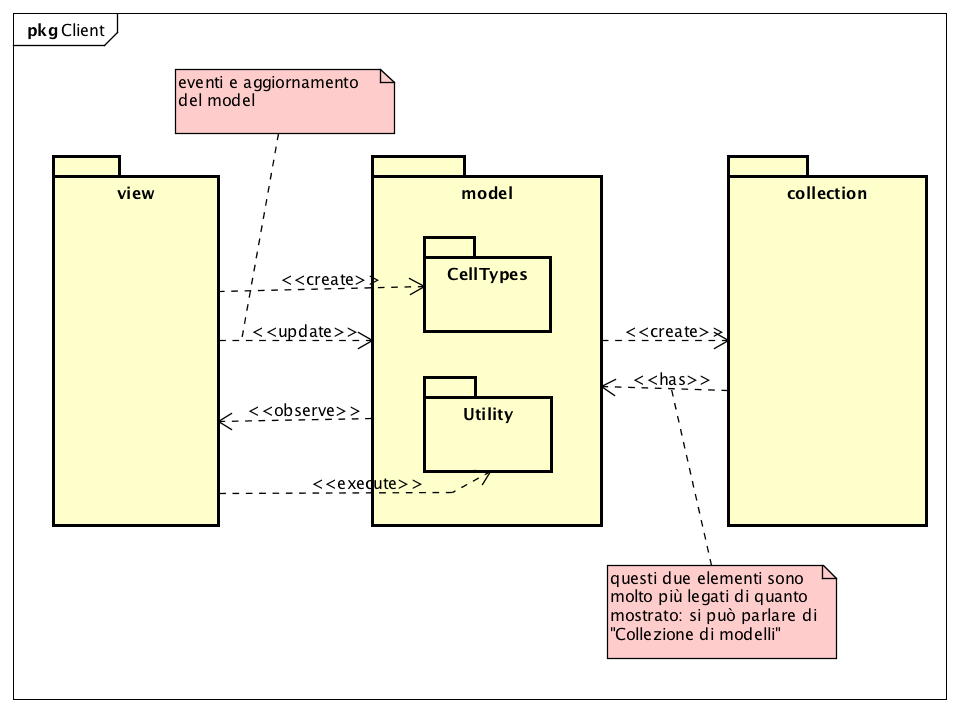
\includegraphics[scale=0.5]{img/client_pkg}
	\caption{Architettura del client.}
\end{figure}



\subsection{Architettura del server} \label{sec:arch_server}
Il server offre tre servizi:
\begin{enumerate}
	\item fornisce al client la pagina HTML dove disegnare i diagrammi;
	\item restituisce l'elenco degli stereotipi esistenti all'interno del server e utilizzabili dal client;
	\item elabora un file JSON in arrivo dal client e gli fornisce l'applicazione generata a partire da tale file.
\end{enumerate}
Questi tre servizi rispettano lo stile architetturale REST (come spiegato più avanti nella sezione \ref{sec:arch_proto}).

Il primo servizio è una semplice pagina HTML, fornita normalmente da Tomcat e arricchita di codice Javascript.

Il secondo e il terzo servizio, invece, sono un programma Java che genera due \emph{servlet}; il programma è organizzato nei seguenti package, come illustrato in figura \ref{fig:server_pkg}:
\begin{itemize}
	\item \textbf{\texttt{controller}} rappresenta il nucleo del \emph{back end}; un \texttt{RequestHandlerController} si occupa di generare le due \emph{servlet} Java, usando \emph{Spring}.
	\item nel package \textbf{\texttt{parser}}, la classe \texttt{Parser} si occupa di convertire il file JSON ricevuto in un oggetto Java di tipo \texttt{ParsedProgram}. Questo oggetto Java rappresenta il programma che l'utente vuole generare; esso si compone di oggetti \texttt{ParsedType} (cioè i tipi definiti dall'utente: gli elementi del diagramma delle classi), i quali si possono comporre di oggetti \texttt{ParsedAttribute} e \texttt{ParsedMethod}; quest'ultimo tipo si compone a sua volta di oggetti \texttt{ParsedInstruction} e così via fino ad arrivare alle istruzioni “atomiche”, come per esempio un \texttt{ParsedReturn}.
	\item \textbf{\texttt{project}} non è altro che il package che organizza i tipi elencati al punto precedente, tutti discendenti da \texttt{ParsedElement}. Inoltre, questo package offre una classe \texttt{ElementFactory}. % che non ho capito cosa fa
	\item \textbf{\texttt{generator}} presenta al suo interno l'interfaccia \texttt{Generator}; le classi che la estendono si occupano di popolare i template \emph{StringTemplate} di un particolare linguaggio di programmazione (\texttt{JavaGenerator} genera codice sorgente Java) e scrivere il risultato su disco. \texttt{GeneratorAssembler} fornisce la giusta implementazione \texttt{Generator}, grazie a un file di configurazione XML e a \emph{Spring}.
	\item \textbf{\texttt{template}} è il package che organizza i template per linguaggio: dall'interfaccia \texttt{Template} discende, ad esempio, \texttt{JavaTemplate}. Anche questo package presenta una classe che si occupa di fornire la giusta implementazione di \texttt{Template}: \texttt{TemplateAssembler}, dipendente anch'esso dal file di configurazione XML.
	\item \textbf{\texttt{stereotype}} espone una classe che recupera da disco i vari template di ogni stereotipo implementato.
	\item \textbf{\texttt{compiler}} presenta l'interfaccia \texttt{Compiler}, le cui implementazioni specifiche (per un certo linguaggio target) compilano il codice sorgente non eseguibile in un programma eseguibile (che viene poi scritto su disco); \texttt{JavaCompiler}, ad esempio, compila codice sorgente Java in \emph{bytecode} per la JVM (Java Virtual Machine) e compatta il codice in un file JAR eseguibile. Anche questo package presenta un \texttt{CompilerAssembler} (dipendente dal file di configurazione XML) che si occupa di fornire la giusta implementazione di \texttt{Compiler}.
	\item \textbf{\texttt{utility}} espone classi di utilità per il programma, come ad esempio una classe \texttt{Compressor} che comprime l'output di un \texttt{Compiler} in formato ZIP. % è pulito tenere un package con un nome così generico?
\end{itemize}

% >>> diagr. dei package del server
\begin{figure} \label{fig:server_pkg}
	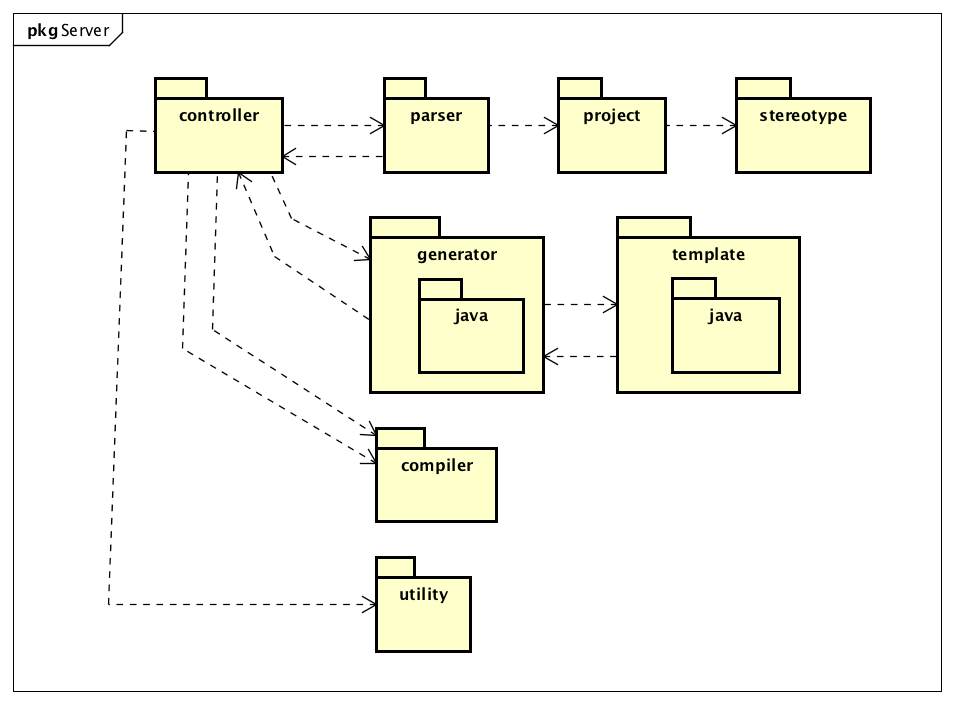
\includegraphics[scale=0.5]{img/server_pkg}
	\caption{Architettura del server.}
\end{figure}



\subsection{Protocollo di comunicazione client-server} \label{sec:arch_proto}
I tre servizi offerti dal server (ottenere la pagina HTML; recuperare stereotipi UML; ottenere l'applicazione generata) seguono lo stile architetturale REST:
\begin{itemize}
	\item La richiesta per ottenere la pagina HTML usa il metodo HTTP GET; la pagina è quindi \emph{cachable} (i router tra client e server possono decidere di ottimizzarne la fornitura).
	\item Il file JSON viene spedito con il metodo HTTP POST, che permette la persistenza di tale file nel server; la persistenza del file JSON è indifferente alla nostra applicazione ma ne aumenta l'estensibilità, in quanto un giorno i manutentori potrebbe voler offrire un servizio di condivisione dei diagrammi disegnati oppure un database di utenti che abbiano i propri diagrammi sul server.
	\item Ognuno dei tre servizi (pagina HTML, recupero di stereotipi e generazione di codice) è una risorsa distinta: questo disaccoppia i due servizi, aumentando ancora la manutenibilità del sistema.
	\item La richiesta per ottenere la pagina HTML è per forza idempotente: lo stato del server non può influire su una pagina statica. %Neanche il recupero di stereotipi dipende dallo stato del server, dato che gli stereotipi sono contenuti in file statici. % <<< o forse no?
	\item La richiesta di generazione di codice è idempotente: l'unica dipendenza esterna al programma è il file JSON, che viene passato dal client.
\end{itemize}

\begin{figure} \label{fig:protocol}
	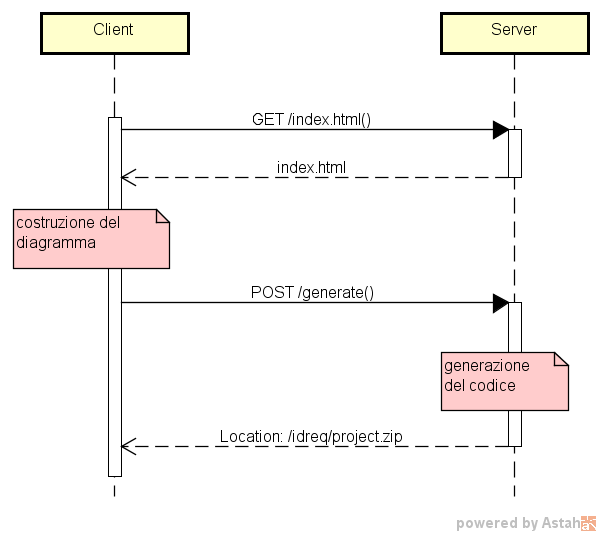
\includegraphics[scale=0.66]{img/http}
	\caption{Possibile interazione tra client e server.}
\end{figure}

% ci sarebbe da fare pure una cosa simile per il recupero degli stereotipi


% ---> distinguere STRUTTURA (classi) da COMPORTAMENTO (procedure)?
% - diagrammi delle classi
% - se serve, qualche diagramma di attività/sequenza
\section{Classi e componenti del \emph{front end}}
%%%%%%%%%%%%%%%%%%%%%%%%%%%%
%%  Componenti del front end
%%%%%%%%%%%%%%%%%%%%%%%%%%%%



\subsection{\nogloxy{swedesigner::client}}
\label{\nogloxy{swedesigner::client}}
\subsubsection{Informazioni generali}
\begin{figure}[H]
	\makebox[\textwidth][c]{
	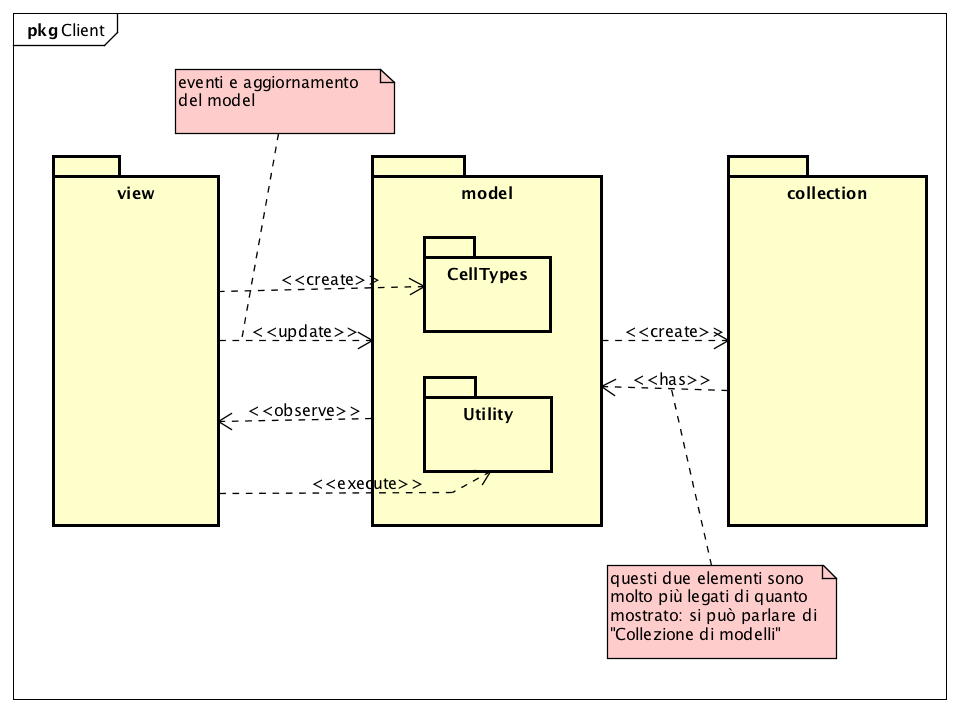
\includegraphics[width=1\textwidth]{img/client_pkg}}
	\caption{Diagramma package client}
\end{figure}
\begin{itemize}
\item \textbf{Descrizione}\\
Questo package descrive le componenti del \emph{front end}, scritte in JavaScript.
\item \textbf{Padre}: \hyperref[\nogloxy{swedesigner}]{\nogloxy{\texttt{swedesigner}}}
\item \textbf{Package contenuti}:
\begin{itemize}
\item \hyperref[\nogloxy{swedesigner::client::model}]{\nogloxy{\texttt{model}}}\\
Questo package contiene i modelli di dati usati dal client per rappresentare l'informazione manipolata dall'utente.
\item \hyperref[\nogloxy{swedesigner::client::view}]{\nogloxy{\texttt{view}}}\\
Questo package raccoglie le classi che rappresentano i menù laterali e il \texttt{canvas} visualizzati dal browser, che popolano template e si sottoscrivono alla view tramite un pattern Observer. (I template non sono contenuti in questo package.)
\end{itemize}
\end{itemize}

\subsection{\nogloxy{swedesigner::client::model}}
\label{\nogloxy{swedesigner::client::model}}
\subsubsection{Informazioni generali}
\begin{figure}[H]
	\makebox[\textwidth][c]{
	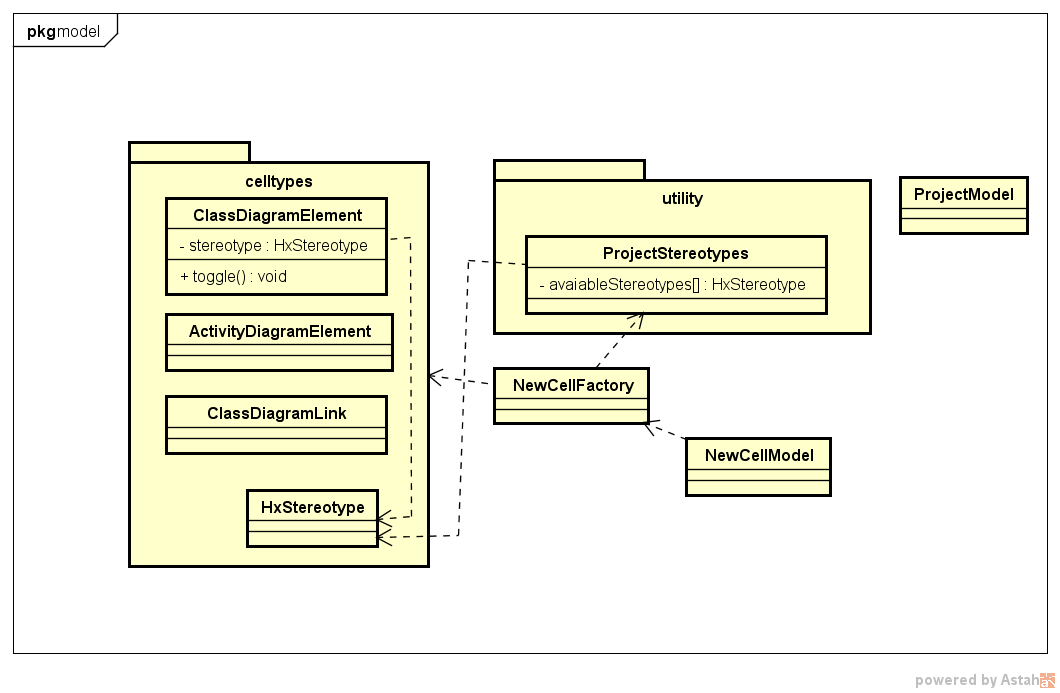
\includegraphics[width=1\textwidth]{img/client_model}}
	\caption{Diagramma package client::model}
\end{figure}
\begin{itemize}
\item \textbf{Descrizione}\\
Questo package contiene i modelli di dati usati dal client per rappresentare l'informazione manipolata dall'utente.
\item \textbf{Padre}: \hyperref[\nogloxy{swedesigner::client}]{\nogloxy{\texttt{client}}}
\item \textbf{Package contenuti}:
\begin{itemize}
\item \hyperref[\nogloxy{swedesigner::client::model::celltypes}]{\nogloxy{\texttt{celltypes}}}\\
Questo package contiene la definizione del modello degli elementi grafici dell'applicazione (e.g. diagrammi delle classi, blocchi condizionali\dots). 
\item \hyperref[\nogloxy{swedesigner::client::model::utility}]{\nogloxy{\texttt{utility}}}\\
Questo package racchiude le classi che definiscono i principali comandi dell'applicazione; esse fanno parte di un unico pattern Command, usato dalla \texttt{AppView} principale.
\end{itemize}
\end{itemize}
\subsubsection{Classi}
\subsubsubsection{\nogloxy{swedesigner::client::model::NewCellFactory}}
\label{\nogloxy{swedesigner::client::model::NewCellFactory}}
\begin{itemize}
\item \textbf{Descrizione}\\
questa classe si occupa di fornire un'istanza di una cella del tipo richiesto da \texttt{NewCellModel}. 
\item \textbf{Utilizzo}\\
viene utilizzata da \texttt{NewCellModel} che richiede una nuova cella (blocco o relazione) per avere un'istanza del blocco richiesto. Il design pattern descritto da questa classe è un Factory Pattern, come spiegato nel libro \emph{Learning Javascript Design Patterns} (\url{addyosmani.com/resources/essentialjsdesignpatterns/book/}).
\item \textbf{Relazioni con altre classi}:
\begin{itemize}
\item \textit{IN} \hyperref[\nogloxy{swedesigner::client::model::celltypes::activity::ActivityDiagramElement}]{\nogloxy{\texttt{ActivityDiagramElement}}}\\
questa classe è la base di tutte le classi che rappresentano i blocchi del diagramma delle attività.
\item \textit{IN} \hyperref[\nogloxy{swedesigner::client::model::NewCellModel}]{\nogloxy{\texttt{NewCellModel}}}\\
questa classe si occupa di fornire tutti i tipi di cell (tutti i blocchi e relazioni) da poter inserire nel diagramma corrente (o classi o attività).
\item \textit{OUT} \hyperref[\nogloxy{swedesigner::client::model::celltypes::class::ClassDiagramElement}]{\nogloxy{\texttt{ClassDiagramElement}}}\\
questa classe è la base di tutte le classi che rappresentano gli elementi del diagramma delle classi.
\end{itemize}
\end{itemize}

\subsubsubsection{\nogloxy{swedesigner::client::model::NewCellModel}}
\label{\nogloxy{swedesigner::client::model::NewCellModel}}
\begin{itemize}
\item \textbf{Descrizione}\\
questa classe si occupa di fornire tutti i tipi di cell (tutti i blocchi e relazioni) da poter inserire nel diagramma corrente (o classi o attività).
\item \textbf{Utilizzo}\\
utilizza \texttt{NewCellFactory} per recuperare una cell del tipo richiesto da \texttt{NewCellView}. Quest'ultima utilizza \texttt{NewCellModel} come modello da dove recuperare tutti i blocchi/relazioni che l'utente può inserire nel diagramma corrente.
\item \textbf{Relazioni con altre classi}:
\begin{itemize}
\item \textit{IN} \hyperref[\nogloxy{swedesigner::client::view::NewCellView}]{\nogloxy{\texttt{NewCellView}}}\\
questa classe si occupa di visualizzare tutti i possibili blocchi e relazioni che si possono inserire nel diagramma delle classi o delle attività.
\item \textit{OUT} \hyperref[\nogloxy{swedesigner::client::model::NewCellFactory}]{\nogloxy{\texttt{NewCellFactory}}}\\
questa classe si occupa di fornire un'istanza di una cella del tipo richiesto da \texttt{NewCellModel}. 
\end{itemize}
\end{itemize}

\subsubsubsection{\nogloxy{swedesigner::client::model::ProjectCommand}}
\label{\nogloxy{swedesigner::client::model::ProjectCommand}}
\begin{itemize}
\item \textbf{Descrizione}\\
questa interfaccia descrive la struttura di un comando che viene chiamato da \texttt{AppView} quando l'utente decide di creare un nuovo progetto, di caricarne uno esistente, di salvarlo o di generare il codice dal diagramma. Il pattern realizzato è il pattern Command.
\item \textbf{Utilizzo}\\
viene utilizzata da \texttt{AppView}, la quale poi chiederà comandi concreti in base all'input richiesto dall'utente.
\item \textbf{Relazioni con altre classi}:
\begin{itemize}
\item \textit{IN} \hyperref[\nogloxy{swedesigner::client::view::AppView}]{\nogloxy{\texttt{AppView}}}\\
questa classe si occupa di gestire l'intera view dell'applicazione, componendo l'interfaccia principale e richiamando le altre view tramite il sistema a template di \backbonejs{}.
\item \textit{OUT} \hyperref[\nogloxy{swedesigner::client::model::ProjectModel}]{\nogloxy{\texttt{ProjectModel}}}\\
questa classe ci permette di aggiungere della logica alla collezione di tutti i diagrammi che possediamo.
\end{itemize}
\end{itemize}

\subsubsubsection{\nogloxy{swedesigner::client::model::ProjectModel}}
\label{\nogloxy{swedesigner::client::model::ProjectModel}}
\begin{itemize}
\item \textbf{Descrizione}\\
questa classe ci permette di aggiungere della logica alla collezione di tutti i diagrammi che possediamo.
\item \textbf{Utilizzo}\\
essa è istanziata da \texttt{ProjectView} e possiede \texttt{DiagramCollection}. È possibile interagire con questo modello anche tramite \texttt{ProjectCommand}, per permettere l'implementazione di funzionalità globali dell'applicazione (e.g. salvataggio e caricamento).
\item \textbf{Relazioni con altre classi}:
\begin{itemize}
\item \textit{IN} \hyperref[\nogloxy{swedesigner::client::model::ProjectCommand}]{\nogloxy{\texttt{ProjectCommand}}}\\
questa interfaccia descrive la struttura di un comando che viene chiamato da \texttt{AppView} quando l'utente decide di creare un nuovo progetto, di caricarne uno esistente, di salvarlo o di generare il codice dal diagramma. Il pattern realizzato è il pattern Command.
\item \textit{IN} \hyperref[\nogloxy{swedesigner::client::view::AppView}]{\nogloxy{\texttt{AppView}}}\\
questa classe si occupa di gestire l'intera view dell'applicazione, componendo l'interfaccia principale e richiamando le altre view tramite il sistema a template di \backbonejs{}.
\item \textit{IN} \hyperref[\nogloxy{swedesigner::client::view::ProjectView}]{\nogloxy{\texttt{ProjectView}}}\\
questa classe rappresenta l'area di disegno principale dell'applicazione, che necessita di essere cambiata tra diagramma delle classi e diagramma delle attività. 
\end{itemize}
\end{itemize}
\subsection{\nogloxy{swedesigner::client::model::celltypes}}
\label{\nogloxy{swedesigner::client::model::celltypes}}
\subsubsection{Informazioni generali}
\begin{figure}[H]
	\makebox[\textwidth][c]{
	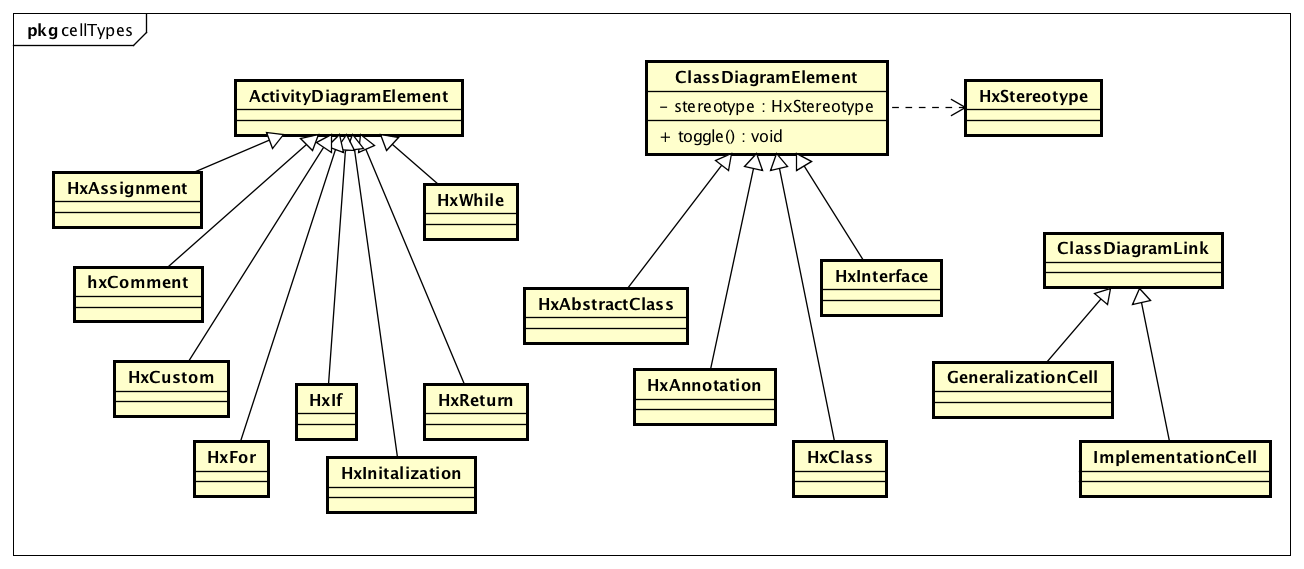
\includegraphics[width=1\textwidth]{img/client_cellTypes}}
	\caption{Diagramma package client::model::celltypes}
\end{figure}
\begin{itemize}
\item \textbf{Descrizione}\\
Questo package contiene la definizione del modello degli elementi grafici dell'applicazione (e.g. diagrammi delle classi, blocchi condizionali\dots). 
\item \textbf{Padre}: \hyperref[\nogloxy{swedesigner::client::model}]{\nogloxy{\texttt{model}}}
\item \textbf{Package contenuti}:
\begin{itemize}
\item \hyperref[\nogloxy{swedesigner::client::model::celltypes::activity}]{\nogloxy{\texttt{activity}}}\\
Questo package contiene la definizione del modello degli elementi specifi del diagramma delle classi dell'applicazione.
\item \hyperref[\nogloxy{swedesigner::client::model::celltypes::class}]{\nogloxy{\texttt{class}}}\\
Questo package contiene la definizione del modello degli elementi specifi del diagramma delle classi dell'applicazione.
\end{itemize}
\end{itemize}
\subsubsection{Classi}
\subsubsubsection{\nogloxy{swedesigner::client::model::celltypes::HxStereotype}}
\label{\nogloxy{swedesigner::client::model::celltypes::HxStereotype}}
\begin{itemize}
\item \textbf{Descrizione}\\
questa classe rappresenta le caratteristiche dello stereotipo che viene assegnato ad un \texttt{ClassDiagramElement} come i meta-attributi e meta-metodi, i quali sono essere ridefiniti dalla classe o interfaccia implementata tramite \proj{}. 
\item \textbf{Utilizzo}\\
ogni elemento possiederà un unico stereotipo per semplificare l'implementazione di \proj{}. Gli stereotipi disponibili sono presenti all'interno della classe \texttt{ProjectStereotypes} (all'interno di \emph{model::utility}).
\item \textbf{Relazioni con altre classi}:
\begin{itemize}
\item \textit{IN} \hyperref[\nogloxy{swedesigner::client::model::celltypes::class::ClassDiagramElement}]{\nogloxy{\texttt{ClassDiagramElement}}}\\
questa classe è la base di tutte le classi che rappresentano gli elementi del diagramma delle classi.
\item \textit{IN} \hyperref[\nogloxy{swedesigner::client::model::utility::ProjectStereotypes}]{\nogloxy{\texttt{ProjectStereotypes}}}\\
questa classe contiene al suo interno i possibili stereotipi utilizzabili recuperati dal server in modo asincrono. Conterrà una lista di elementi \textt{HxStereotype}.
\end{itemize}
\end{itemize}
\subsection{\nogloxy{swedesigner::client::model::celltypes::activity}}
\label{\nogloxy{swedesigner::client::model::celltypes::activity}}
\subsubsection{Informazioni generali}
\begin{itemize}
\item \textbf{Descrizione}\\
Questo package contiene la definizione del modello degli elementi specifi del diagramma delle classi dell'applicazione.
\item \textbf{Padre}: \hyperref[\nogloxy{swedesigner::client::model::celltypes}]{\nogloxy{\texttt{celltypes}}}
\end{itemize}
\subsubsection{Classi}
\subsubsubsection{\nogloxy{swedesigner::client::model::celltypes::activity::ActivityDiagramElement}}
\label{\nogloxy{swedesigner::client::model::celltypes::activity::ActivityDiagramElement}}
\begin{itemize}
\item \textbf{Descrizione}\\
questa classe è la base di tutte le classi che rappresentano i blocchi del diagramma delle attività.
\item \textbf{Utilizzo}\\
estende sottotipi della classe \texttt{Element} (la quale deriva a sua volta da \texttt{Cell})  di \jointjs{} e viene estesa da tutte le classi specifiche di ogni blocco del diagramma delle attività. Questa classe è indirettamente correlata a \texttt{NewCellFactory}.
\item \textbf{Sottoclassi}:
\begin{itemize}
\item \hyperref[\nogloxy{swedesigner::client::model::celltypes::activity::HxCustom}]{\nogloxy{\texttt{HxCustom}}}
\item \hyperref[\nogloxy{swedesigner::client::model::celltypes::activity::HxElse}]{\nogloxy{\texttt{HxElse}}}
\item \hyperref[\nogloxy{swedesigner::client::model::celltypes::activity::HxFor}]{\nogloxy{\texttt{HxFor}}}
\item \hyperref[\nogloxy{swedesigner::client::model::celltypes::activity::HxIf}]{\nogloxy{\texttt{HxIf}}}
\item \hyperref[\nogloxy{swedesigner::client::model::celltypes::activity::HxReturn}]{\nogloxy{\texttt{HxReturn}}}
\item \hyperref[\nogloxy{swedesigner::client::model::celltypes::activity::HxVariable}]{\nogloxy{\texttt{HxVariable}}}
\item \hyperref[\nogloxy{swedesigner::client::model::celltypes::activity::HxWhile}]{\nogloxy{\texttt{HxWhile}}}
\end{itemize}
\item \textbf{Relazioni con altre classi}:
\begin{itemize}
\item \textit{OUT} \hyperref[\nogloxy{swedesigner::client::model::NewCellFactory}]{\nogloxy{\texttt{NewCellFactory}}}\\
questa classe si occupa di fornire un'istanza di una cella del tipo richiesto da \texttt{NewCellModel}. 
\end{itemize}
\end{itemize}

\subsubsubsection{\nogloxy{swedesigner::client::model::celltypes::activity::HxCustom}}
\label{\nogloxy{swedesigner::client::model::celltypes::activity::HxCustom}}
\begin{itemize}
\item \textbf{Descrizione}\\
questa classe rappresenta il blocco custom del diagramma delle attività che permette all'utente di inserire liberamente codice nel linguaggio target scelto.
\item \textbf{Utilizzo}\\
la classe \texttt{NewCellFactory} ritorna un'istanza di questa classe ogni volta che l'utente richiede un nuovo blocco di codice personalizzato.
\item \textbf{Classi ereditate}:
\begin{itemize}
\item \hyperref[\nogloxy{swedesigner::client::model::celltypes::activity::ActivityDiagramElement}]{\nogloxy{\texttt{ActivityDiagramElement}}}
\end{itemize}
\end{itemize}

\subsubsubsection{\nogloxy{swedesigner::client::model::celltypes::activity::HxElse}}
\label{\nogloxy{swedesigner::client::model::celltypes::activity::HxElse}}
\begin{itemize}
\item \textbf{Descrizione}\\
Questa classe rappresenta il blocco else del diagramma delle attività
\item \textbf{Utilizzo}\\
la classe \texttt{NewCellFactory} ritorna un'istanza di questa classe ogni volta che l'utente richiede un nuovo blocco \texttt{for}.
\item \textbf{Classi ereditate}:
\begin{itemize}
\item \hyperref[\nogloxy{swedesigner::client::model::celltypes::activity::ActivityDiagramElement}]{\nogloxy{\texttt{ActivityDiagramElement}}}
\end{itemize}
\end{itemize}

\subsubsubsection{\nogloxy{swedesigner::client::model::celltypes::activity::HxFor}}
\label{\nogloxy{swedesigner::client::model::celltypes::activity::HxFor}}
\begin{itemize}
\item \textbf{Descrizione}\\
questa classe rappresenta il blocco \texttt{for} del diagramma delle attività.
\item \textbf{Utilizzo}\\
la classe \texttt{NewCellFactory} ritorna un'istanza di questa classe ogni volta che l'utente richiede un nuovo blocco \texttt{for}.
\item \textbf{Classi ereditate}:
\begin{itemize}
\item \hyperref[\nogloxy{swedesigner::client::model::celltypes::activity::ActivityDiagramElement}]{\nogloxy{\texttt{ActivityDiagramElement}}}
\end{itemize}
\end{itemize}

\subsubsubsection{\nogloxy{swedesigner::client::model::celltypes::activity::HxIf}}
\label{\nogloxy{swedesigner::client::model::celltypes::activity::HxIf}}
\begin{itemize}
\item \textbf{Descrizione}\\
questa classe rappresenta il blocco \texttt{if} del diagramma delle attività.
\item \textbf{Utilizzo}\\
la classe \texttt{NewCellFactory} ritorna un'istanza di questa classe ogni volta che l'utente richiede un nuovo blocco \texttt{if}.
\item \textbf{Classi ereditate}:
\begin{itemize}
\item \hyperref[\nogloxy{swedesigner::client::model::celltypes::activity::ActivityDiagramElement}]{\nogloxy{\texttt{ActivityDiagramElement}}}
\end{itemize}
\end{itemize}

\subsubsubsection{\nogloxy{swedesigner::client::model::celltypes::activity::HxReturn}}
\label{\nogloxy{swedesigner::client::model::celltypes::activity::HxReturn}}
\begin{itemize}
\item \textbf{Descrizione}\\
questa classe rappresenta il blocco \emph{return} del diagramma delle attività.
\item \textbf{Utilizzo}\\
la classe \texttt{NewCellFactory} ritorna un'istanza di questa classe ogni volta che l'utente richiede un nuovo blocco \emph{return}.
\item \textbf{Classi ereditate}:
\begin{itemize}
\item \hyperref[\nogloxy{swedesigner::client::model::celltypes::activity::ActivityDiagramElement}]{\nogloxy{\texttt{ActivityDiagramElement}}}
\end{itemize}
\end{itemize}

\subsubsubsection{\nogloxy{swedesigner::client::model::celltypes::activity::HxVariable}}
\label{\nogloxy{swedesigner::client::model::celltypes::activity::HxVariable}}
\begin{itemize}
\item \textbf{Descrizione}\\
questa classe rappresenta il blocco di assegnazione o inizializzazione di una variabile o di chiamata di un metodo del diagramma delle attività.
\item \textbf{Utilizzo}\\
la classe \texttt{NewCellFactory} ritorna un'istanza di questa classe ogni volta che l'utente richiede un nuovo blocco variabile.
\item \textbf{Classi ereditate}:
\begin{itemize}
\item \hyperref[\nogloxy{swedesigner::client::model::celltypes::activity::ActivityDiagramElement}]{\nogloxy{\texttt{ActivityDiagramElement}}}
\end{itemize}
\end{itemize}

\subsubsubsection{\nogloxy{swedesigner::client::model::celltypes::activity::HxWhile}}
\label{\nogloxy{swedesigner::client::model::celltypes::activity::HxWhile}}
\begin{itemize}
\item \textbf{Descrizione}\\
questa classe rappresenta il blocco \emph{while} del diagramma delle attività.
\item \textbf{Utilizzo}\\
la classe \texttt{NewCellFactory} ritorna un'istanza di questa classe ogni volta che l'utente richiede un nuovo blocco \emph{while}.
\item \textbf{Classi ereditate}:
\begin{itemize}
\item \hyperref[\nogloxy{swedesigner::client::model::celltypes::activity::ActivityDiagramElement}]{\nogloxy{\texttt{ActivityDiagramElement}}}
\end{itemize}
\end{itemize}
\subsection{\nogloxy{swedesigner::client::model::celltypes::class}}
\label{\nogloxy{swedesigner::client::model::celltypes::class}}
\subsubsection{Informazioni generali}
\begin{itemize}
\item \textbf{Descrizione}\\
Questo package contiene la definizione del modello degli elementi specifi del diagramma delle classi dell'applicazione.
\item \textbf{Padre}: \hyperref[\nogloxy{swedesigner::client::model::celltypes}]{\nogloxy{\texttt{celltypes}}}
\end{itemize}
\subsubsection{Classi}
\subsubsubsection{\nogloxy{swedesigner::client::model::celltypes::class::ClassDiagramElement}}
\label{\nogloxy{swedesigner::client::model::celltypes::class::ClassDiagramElement}}
\begin{itemize}
\item \textbf{Descrizione}\\
questa classe è la base di tutte le classi che rappresentano gli elementi del diagramma delle classi.
\item \textbf{Utilizzo}\\
eredita da sottotipi della classe \texttt{Element} di \jointjs{} (la quale deriva a sua volta da \texttt{Cell}) e viene estesa da tutte le classi specifiche di ogni blocco del diagramma delle classi. Questa classe è indirettamente correlata con \texttt{NewCellFactory}, derivando da \texttt{Cell}.
\item \textbf{Sottoclassi}:
\begin{itemize}
\item \hyperref[\nogloxy{swedesigner::client::model::celltypes::class::HxClass}]{\nogloxy{\texttt{HxClass}}}
\item \hyperref[\nogloxy{swedesigner::client::model::celltypes::class::HxInterface}]{\nogloxy{\texttt{HxInterface}}}
\end{itemize}
\item \textbf{Relazioni con altre classi}:
\begin{itemize}
\item \textit{IN} \hyperref[\nogloxy{swedesigner::client::model::NewCellFactory}]{\nogloxy{\texttt{NewCellFactory}}}\\
questa classe si occupa di fornire un'istanza di una cella del tipo richiesto da \texttt{NewCellModel}. 
\item \textit{OUT} \hyperref[\nogloxy{swedesigner::client::model::celltypes::HxStereotype}]{\nogloxy{\texttt{HxStereotype}}}\\
questa classe rappresenta le caratteristiche dello stereotipo che viene assegnato ad un \texttt{ClassDiagramElement} come i meta-attributi e meta-metodi, i quali sono essere ridefiniti dalla classe o interfaccia implementata tramite \proj{}. 
\end{itemize}
\end{itemize}

\subsubsubsection{\nogloxy{swedesigner::client::model::celltypes::class::ClassDiagramLink}}
\label{\nogloxy{swedesigner::client::model::celltypes::class::ClassDiagramLink}}
\begin{itemize}
\item \textbf{Descrizione}\\
questa classe è la base di tutte le classi che rappresentano le relazioni tra gli elementi del diagramma delle classi.
\item \textbf{Utilizzo}\\
eredita dalla classe \texttt{Link} di \jointjs{} e viene estesa da tutte le classi specifiche di ogni relazione del diagramma delle classi.
\item \textbf{Sottoclassi}:
\begin{itemize}
\item \hyperref[\nogloxy{swedesigner::client::model::celltypes::class::HxAssociation}]{\nogloxy{\texttt{HxAssociation}}}
\item \hyperref[\nogloxy{swedesigner::client::model::celltypes::class::HxGeneralization}]{\nogloxy{\texttt{HxGeneralization}}}
\item \hyperref[\nogloxy{swedesigner::client::model::celltypes::class::HxImplementation}]{\nogloxy{\texttt{HxImplementation}}}
\end{itemize}
\end{itemize}

\subsubsubsection{\nogloxy{swedesigner::client::model::celltypes::class::HxAssociation}}
\label{\nogloxy{swedesigner::client::model::celltypes::class::HxAssociation}}
\begin{itemize}
\item \textbf{Descrizione}\\
Questa classe rappresenta una relazione associazione tra due blocchi del diagramma delle classi
\item \textbf{Utilizzo}\\
eredita dalla classe \texttt{ClassDiagramLink}. È indirettamente collegata a \texttt{NewCellFactory} in quanto è anch'essa una derivata di \texttt{Cell}.
\item \textbf{Classi ereditate}:
\begin{itemize}
\item \hyperref[\nogloxy{swedesigner::client::model::celltypes::class::ClassDiagramLink}]{\nogloxy{\texttt{ClassDiagramLink}}}
\end{itemize}
\end{itemize}

\subsubsubsection{\nogloxy{swedesigner::client::model::celltypes::class::HxClass}}
\label{\nogloxy{swedesigner::client::model::celltypes::class::HxClass}}
\begin{itemize}
\item \textbf{Descrizione}\\
questa classe rappresenta il blocco \texttt{class} del diagramma delle classi UML.
\item \textbf{Utilizzo}\\
la classe \texttt{NewCellFactory} ritorna un'istanza di questa classe ogni volta che l'utente richiede un nuovo elemento \emph{class}.
\item \textbf{Classi ereditate}:
\begin{itemize}
\item \hyperref[\nogloxy{swedesigner::client::model::celltypes::class::ClassDiagramElement}]{\nogloxy{\texttt{ClassDiagramElement}}}
\end{itemize}
\end{itemize}

\subsubsubsection{\nogloxy{swedesigner::client::model::celltypes::class::HxComment}}
\label{\nogloxy{swedesigner::client::model::celltypes::class::HxComment}}
\begin{itemize}
\item \textbf{Descrizione}\\
questa classe rappresenta la cella di commento del diagramma delle classi UML. Eredita da un tipo base di jointjs.
\item \textbf{Utilizzo}\\
la classe \texttt{NewCellFactory} ritorna un'istanza di questa classe ogni volta che l'utente richiede un nuovo commento.
\end{itemize}

\subsubsubsection{\nogloxy{swedesigner::client::model::celltypes::class::HxGeneralization}}
\label{\nogloxy{swedesigner::client::model::celltypes::class::HxGeneralization}}
\begin{itemize}
\item \textbf{Descrizione}\\
questa classe rappresenta la relazione di generalizzazione tra due celle del diagramma delle classi.
\item \textbf{Utilizzo}\\
eredita dalla classe \texttt{ClassDiagramLink}. È indirettamente collegata a \texttt{NewCellFactory} in quanto è anch'essa una derivata di \texttt{Cell}.
\item \textbf{Classi ereditate}:
\begin{itemize}
\item \hyperref[\nogloxy{swedesigner::client::model::celltypes::class::ClassDiagramLink}]{\nogloxy{\texttt{ClassDiagramLink}}}
\end{itemize}
\end{itemize}

\subsubsubsection{\nogloxy{swedesigner::client::model::celltypes::class::HxImplementation}}
\label{\nogloxy{swedesigner::client::model::celltypes::class::HxImplementation}}
\begin{itemize}
\item \textbf{Descrizione}\\
questa classe rappresenta la relazione di implementazione tra due celle del diagramma delle classi.
\item \textbf{Utilizzo}\\
eredita dalla classe \texttt{ClassDiagramLink}. È indirettamente collegata a \texttt{NewCellFactory} in quanto è anch'essa una derivata di \texttt{Cell}.
\item \textbf{Classi ereditate}:
\begin{itemize}
\item \hyperref[\nogloxy{swedesigner::client::model::celltypes::class::ClassDiagramLink}]{\nogloxy{\texttt{ClassDiagramLink}}}
\end{itemize}
\end{itemize}

\subsubsubsection{\nogloxy{swedesigner::client::model::celltypes::class::HxInterface}}
\label{\nogloxy{swedesigner::client::model::celltypes::class::HxInterface}}
\begin{itemize}
\item \textbf{Descrizione}\\
questa classe rappresenta il costrutto \emph{interface} del diagramma delle classi UML.
\item \textbf{Utilizzo}\\
la classe \texttt{NewCellFactory} ritorna un'istanza di questa classe ogni volta che l'utente richiede un nuovo elemento \emph{interface}.
\item \textbf{Classi ereditate}:
\begin{itemize}
\item \hyperref[\nogloxy{swedesigner::client::model::celltypes::class::ClassDiagramElement}]{\nogloxy{\texttt{ClassDiagramElement}}}
\end{itemize}
\end{itemize}
\subsection{\nogloxy{swedesigner::client::model::utility}}
\label{\nogloxy{swedesigner::client::model::utility}}
\subsubsection{Informazioni generali}
\begin{figure}[H]
	\makebox[\textwidth][c]{
	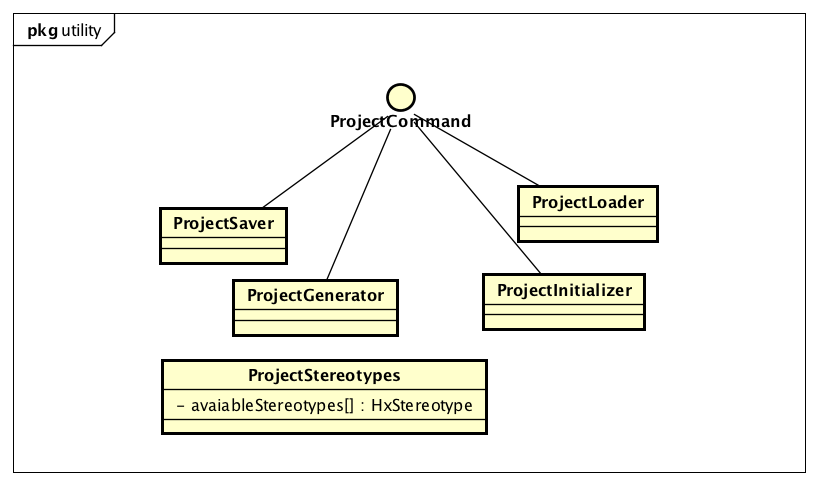
\includegraphics[width=1\textwidth]{img/client_utility}}
	\caption{Diagramma package client::model::utility}
\end{figure}
\begin{itemize}
\item \textbf{Descrizione}\\
Questo package racchiude le classi che definiscono i principali comandi dell'applicazione; esse fanno parte di un unico pattern Command, usato dalla \texttt{AppView} principale.
\item \textbf{Padre}: \hyperref[\nogloxy{swedesigner::client::model}]{\nogloxy{\texttt{model}}}
\end{itemize}
\subsubsection{Classi}
\subsubsubsection{\nogloxy{swedesigner::client::model::utility::ProjectStereotypes}}
\label{\nogloxy{swedesigner::client::model::utility::ProjectStereotypes}}
\begin{itemize}
\item \textbf{Descrizione}\\
questa classe contiene al suo interno i possibili stereotipi utilizzabili recuperati dal server in modo asincrono. Conterrà una lista di elementi \textt{HxStereotype}.
\item \textbf{Utilizzo}\\
\texttt{DetailsView} necessita degli stereotipi esistenti per permettere l'inserimento e la modifica dello stereotipo di una classe. È possibile che la \texttt{NewCellFactory} faccia una richiesta simile a questa classe, al fine di poter fornire all'utente la possibilità di inserire una classe già stereotipata. 
\item \textbf{Relazioni con altre classi}:
\begin{itemize}
\item \textit{IN} \hyperref[\nogloxy{swedesigner::client::view::DetailsView}]{\nogloxy{\texttt{DetailsView}}}\\
questa classe si occupa di visualizzare tutti i campi di un blocco o di una relazione (come il nome di una classe, i suoi attributi, la condizione di un blocco \texttt{if} o il blocco di partenza di una relazione) permettendone anche la modifica. È possibile anche specificare uno stereotipo per la classe.

\item \textit{OUT} \hyperref[\nogloxy{swedesigner::client::model::celltypes::HxStereotype}]{\nogloxy{\texttt{HxStereotype}}}\\
questa classe rappresenta le caratteristiche dello stereotipo che viene assegnato ad un \texttt{ClassDiagramElement} come i meta-attributi e meta-metodi, i quali sono essere ridefiniti dalla classe o interfaccia implementata tramite \proj{}. 
\end{itemize}
\end{itemize}
\subsection{\nogloxy{swedesigner::client::view}}
\label{\nogloxy{swedesigner::client::view}}
\subsubsection{Informazioni generali}
\begin{figure}[H]
	\makebox[\textwidth][c]{
	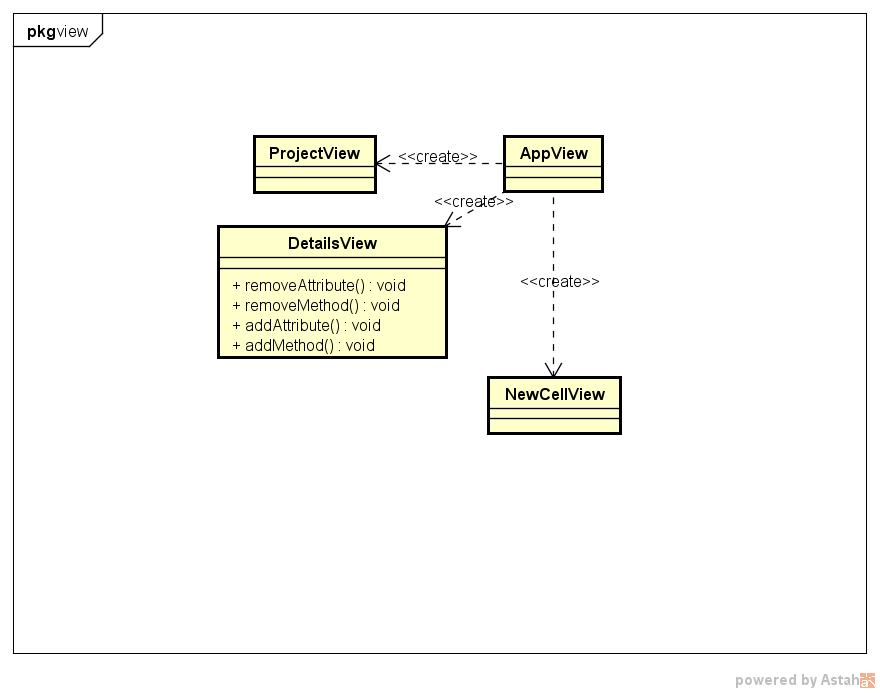
\includegraphics[width=1\textwidth]{img/client_view}}
	\caption{Diagramma package client::view}
\end{figure}
\begin{itemize}
\item \textbf{Descrizione}\\
Questo package raccoglie le classi che rappresentano i menù laterali e il \texttt{canvas} visualizzati dal browser, che popolano template e si sottoscrivono alla view tramite un pattern Observer. (I template non sono contenuti in questo package.)
\item \textbf{Padre}: \hyperref[\nogloxy{swedesigner::client}]{\nogloxy{\texttt{client}}}
\end{itemize}
\subsubsection{Classi}
\subsubsubsection{\nogloxy{swedesigner::client::view::AppView}}
\label{\nogloxy{swedesigner::client::view::AppView}}
\begin{itemize}
\item \textbf{Descrizione}\\
questa classe si occupa di gestire l'intera view dell'applicazione, componendo l'interfaccia principale e richiamando le altre view tramite il sistema a template di \backbonejs{}.
\item \textbf{Utilizzo}\\
essa è la prima classe costruita dall'entry point del programma.
\item \textbf{Relazioni con altre classi}:
\begin{itemize}
\item \textit{OUT} \hyperref[\nogloxy{swedesigner::client::model::ProjectCommand}]{\nogloxy{\texttt{ProjectCommand}}}\\
questa interfaccia descrive la struttura di un comando che viene chiamato da \texttt{AppView} quando l'utente decide di creare un nuovo progetto, di caricarne uno esistente, di salvarlo o di generare il codice dal diagramma. Il pattern realizzato è il pattern Command.
\item \textit{OUT} \hyperref[\nogloxy{swedesigner::client::model::ProjectModel}]{\nogloxy{\texttt{ProjectModel}}}\\
questa classe ci permette di aggiungere della logica alla collezione di tutti i diagrammi che possediamo.
\item \textit{OUT} \hyperref[\nogloxy{swedesigner::client::view::DetailsView}]{\nogloxy{\texttt{DetailsView}}}\\
questa classe si occupa di visualizzare tutti i campi di un blocco o di una relazione (come il nome di una classe, i suoi attributi, la condizione di un blocco \texttt{if} o il blocco di partenza di una relazione) permettendone anche la modifica. È possibile anche specificare uno stereotipo per la classe.

\item \textit{OUT} \hyperref[\nogloxy{swedesigner::client::view::NewCellView}]{\nogloxy{\texttt{NewCellView}}}\\
questa classe si occupa di visualizzare tutti i possibili blocchi e relazioni che si possono inserire nel diagramma delle classi o delle attività.
\item \textit{OUT} \hyperref[\nogloxy{swedesigner::client::view::ProjectView}]{\nogloxy{\texttt{ProjectView}}}\\
questa classe rappresenta l'area di disegno principale dell'applicazione, che necessita di essere cambiata tra diagramma delle classi e diagramma delle attività. 
\end{itemize}
\end{itemize}

\subsubsubsection{\nogloxy{swedesigner::client::view::DetailsView}}
\label{\nogloxy{swedesigner::client::view::DetailsView}}
\begin{itemize}
\item \textbf{Descrizione}\\
questa classe si occupa di visualizzare tutti i campi di un blocco o di una relazione (come il nome di una classe, i suoi attributi, la condizione di un blocco \texttt{if} o il blocco di partenza di una relazione) permettendone anche la modifica. È possibile anche specificare uno stereotipo per la classe.

\item \textbf{Utilizzo}\\
utilizza come model una tra le classi contenute nel package \texttt{celltypes}, in base alla selezione fatta dall'utente, e ne modifica i campi in base all'input. Essa eredita dalla \texttt{View} di \emph{Backbone.js} ed è una \emph{view} parallela alla \texttt{CellView} di ogni \texttt{Cell}, in quanto usa gli stessi modelli mostrando diversamente i dati.
In futuro, qualora l'implementazione di questa classe risulti troppo pesante o complicata da testare, è possibile subclassare questa classe in \emph{view} multiple e prevedere una nuova \emph{factory} di view.
\item \textbf{Relazioni con altre classi}:
\begin{itemize}
\item \textit{IN} \hyperref[\nogloxy{swedesigner::client::view::AppView}]{\nogloxy{\texttt{AppView}}}\\
questa classe si occupa di gestire l'intera view dell'applicazione, componendo l'interfaccia principale e richiamando le altre view tramite il sistema a template di \backbonejs{}.
\item \textit{OUT} \hyperref[\nogloxy{swedesigner::client::model::utility::ProjectStereotypes}]{\nogloxy{\texttt{ProjectStereotypes}}}\\
questa classe contiene al suo interno i possibili stereotipi utilizzabili recuperati dal server in modo asincrono. Conterrà una lista di elementi \textt{HxStereotype}.
\end{itemize}
\end{itemize}

\subsubsubsection{\nogloxy{swedesigner::client::view::NewCellView}}
\label{\nogloxy{swedesigner::client::view::NewCellView}}
\begin{itemize}
\item \textbf{Descrizione}\\
questa classe si occupa di visualizzare tutti i possibili blocchi e relazioni che si possono inserire nel diagramma delle classi o delle attività.
\item \textbf{Utilizzo}\\
utilizza \texttt{NewCellModel} per recuperare i blocchi e relazioni inseribili nel diagramma corrente (che può essere o delle classi o delle attività).
\item \textbf{Relazioni con altre classi}:
\begin{itemize}
\item \textit{IN} \hyperref[\nogloxy{swedesigner::client::view::AppView}]{\nogloxy{\texttt{AppView}}}\\
questa classe si occupa di gestire l'intera view dell'applicazione, componendo l'interfaccia principale e richiamando le altre view tramite il sistema a template di \backbonejs{}.
\item \textit{OUT} \hyperref[\nogloxy{swedesigner::client::model::NewCellModel}]{\nogloxy{\texttt{NewCellModel}}}\\
questa classe si occupa di fornire tutti i tipi di cell (tutti i blocchi e relazioni) da poter inserire nel diagramma corrente (o classi o attività).
\end{itemize}
\end{itemize}

\subsubsubsection{\nogloxy{swedesigner::client::view::ProjectView}}
\label{\nogloxy{swedesigner::client::view::ProjectView}}
\begin{itemize}
\item \textbf{Descrizione}\\
questa classe rappresenta l'area di disegno principale dell'applicazione, che necessita di essere cambiata tra diagramma delle classi e diagramma delle attività. 
\item \textbf{Utilizzo}\\
seleziona l'elemento \emph{Graph} da visualizzare. esso è presente nel relativo \emph{model}, che sarà di volta in volta cambiato selezionandolo dalla sua \emph{collection}.
\item \textbf{Relazioni con altre classi}:
\begin{itemize}
\item \textit{IN} \hyperref[\nogloxy{swedesigner::client::view::AppView}]{\nogloxy{\texttt{AppView}}}\\
questa classe si occupa di gestire l'intera view dell'applicazione, componendo l'interfaccia principale e richiamando le altre view tramite il sistema a template di \backbonejs{}.
\item \textit{OUT} \hyperref[\nogloxy{swedesigner::client::model::ProjectModel}]{\nogloxy{\texttt{ProjectModel}}}\\
questa classe ci permette di aggiungere della logica alla collezione di tutti i diagrammi che possediamo.
\end{itemize}
\end{itemize}

\begin{adjustwidth}{-3cm}{-3cm}
	\begin{figure}[H]
		\makebox[\textwidth][c]{
		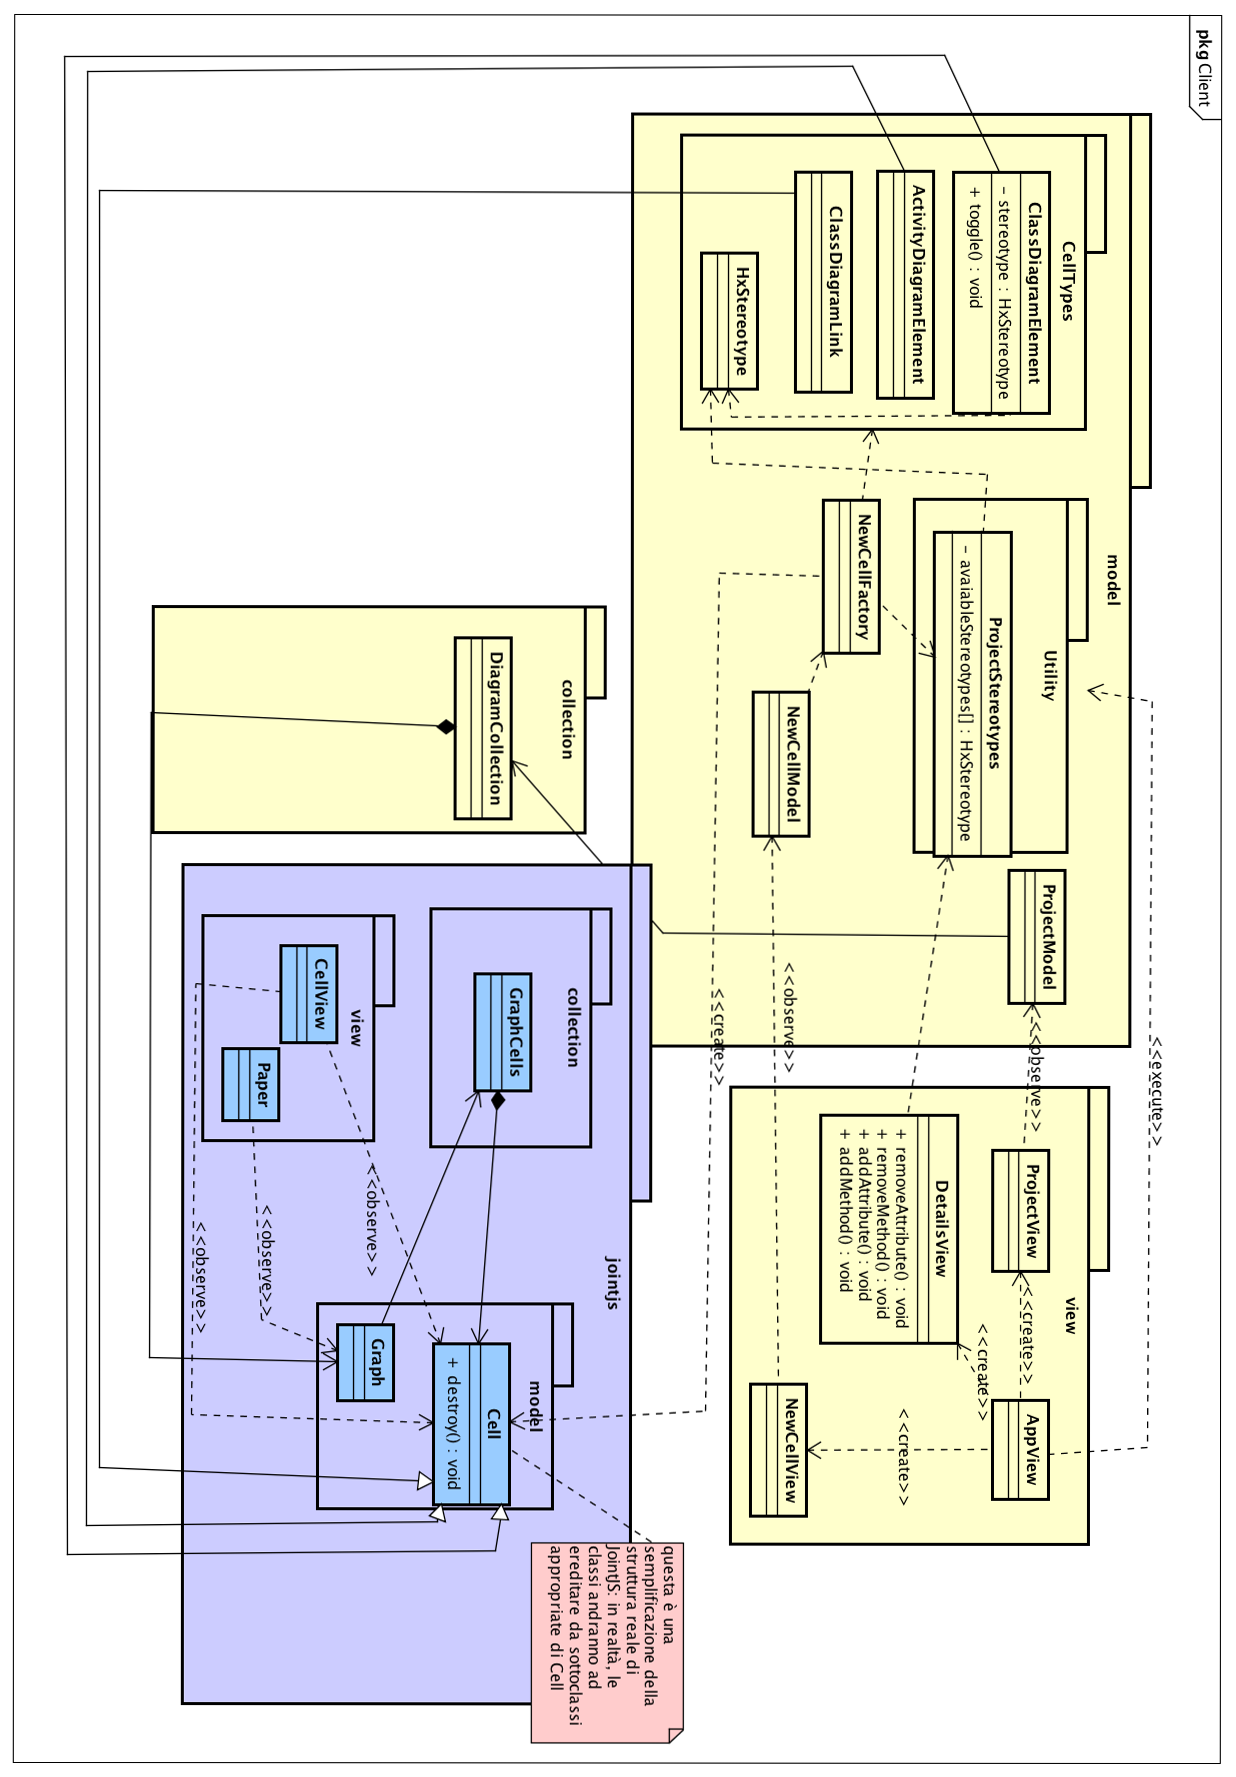
\includegraphics[width=1\textwidth]{img/client_hor}}
		\caption{Diagramma package client}
	\end{figure}
\end{adjustwidth}


\section{Classi e componenti del \emph{back end}}
\subsection{\nogloxy{SWEDesigner::Server}}
\label{\nogloxy{SWEDesigner::Server}}
\subsubsection{Informazioni generali}
\begin{itemize}
\item \textbf{Descrizione}\\
questo package contiene le componenti del server, scritte in Java.
\item \textbf{Padre}: \hyperref[\nogloxy{SWEDesigner}]{\nogloxy{\texttt{SWEDesigner}}}
\item \textbf{Package contenuti}:
\begin{itemize}
\item \hyperref[\nogloxy{SWEDesigner::Server::Compiler}]{\nogloxy{\texttt{Compiler}}}\\
questo package contiene le classi adibite alla compilazione del codice sorgente in eseguibile nel linguaggio target specifico. È stata prevista la possibilità di ampliare questo package inserendo al suo interno ulteriori package. All'interno di questo package è presente unicamente il package \emph{java}.
\item \hyperref[\nogloxy{SWEDesigner::Server::Controller}]{\nogloxy{\texttt{Controller}}}\\
questo package contiene i vari controller che implementano il pattern Front Controller fornito dal framework \spring{}. Ogni controller dovrebbe occuparsi di gestire una richiesta e di rispondere opportunamente ad essa, attraverso il protocollo REST definito.
\item \hyperref[\nogloxy{SWEDesigner::Server::Generator}]{\nogloxy{\texttt{Generator}}}\\
questo package contiene le classi adibite alla trasformazione da programma rappresentato in memoria a codice sorgente, nel linguaggio target specifico. È stata prevista la possibilità di ampliare questo package inserendo al suo interno ulteriori package. All'interno di questo package è presente unicamente il package \emph{java}.
\item \hyperref[\nogloxy{SWEDesigner::Server::Parser}]{\nogloxy{\texttt{Parser}}}\\
al suo interno sono inserite le classi utili all'attività di parsing delle richieste provenienti dai client.
\item \hyperref[\nogloxy{SWEDesigner::Server::Project}]{\nogloxy{\texttt{Project}}}\\
questo package contiene al suo interno le classi utili a rappresentare un progetto. Il package parser necessita di questo package per poter dare in output un programma rappresentato in memoria. Per chiarezza e per evitare l'uso di keyword riservate dal linguaggio Java, all'inizio del nome di queste classi è inserito il prefisso \emph{Parsed} (e.g. \emph{ParsedClass}).
\item \hyperref[\nogloxy{SWEDesigner::Server::Stereotype}]{\nogloxy{\texttt{Stereotype}}}\\
all'interno di questo package sono inserite le classi che descrivono ciò che caratterizza un particolare stereotipo. Queste classi derivano tutte da una classe base, chiamata Stereotype. Le classi che definiscono come deve variare ogni stereotipo sono contraddistinte dal suffisso \emph{Stereotype} (e.g. BoardStereotype). Si noti che tra queste classi non sono presenti dei legami, in quanto queste classi sono necessarie alla generazione del codice. La struttura degli stereotipi assegnabili ad ogni classe e le loro relazioni saranno definite successivamente nella \emph{Definizione di prodotto v 1.0.0}.
\item \hyperref[\nogloxy{SWEDesigner::Server::Template}]{\nogloxy{\texttt{Template}}}\\
questo package contiene le classi necessarie a trasformare l'oggetto che rappresenta il programma in una stringa di testo che rappresenta il codice sorgente tramite un sistema a template, il quale definirà tramite dei file di testo la struttura di ogni componente del programma; per facilitare questo compito sarà usata la libreria \stringtemplate{}. Similarmente al package \emph{Generator} si è prevista la possibilità di implementare un sistema di template per ogni linguaggio, implementando diversamente l'interfaccia della classe Template e definendo un nuovo package (e.g. \emph{Java}).
\item \hyperref[\nogloxy{SWEDesigner::Server::Utility}]{\nogloxy{\texttt{Utility}}}\\
in questo package sono contenute le componenti secondarie necessarie al server, indipendentemente dal linguaggio target dell'applicazione.
\end{itemize}
\end{itemize}

\subsection{\nogloxy{SWEDesigner::Server::Compiler}}
\label{\nogloxy{SWEDesigner::Server::Compiler}}
\subsubsection{Informazioni generali}
\begin{itemize}
\item \textbf{Descrizione}\\
questo package contiene le classi adibite alla compilazione del codice sorgente in eseguibile nel linguaggio target specifico. È stata prevista la possibilità di ampliare questo package inserendo al suo interno ulteriori package. All'interno di questo package è presente unicamente il package \emph{java}.
\item \textbf{Padre}: \hyperref[\nogloxy{SWEDesigner::Server}]{\nogloxy{\texttt{Server}}}
\item \textbf{Package contenuti}:
\begin{itemize}
\item \hyperref[\nogloxy{SWEDesigner::Server::Compiler::Java}]{\nogloxy{\texttt{Java}}}\\
in questo package è descritta l'implementazione dell'interfaccia \emph{Compiler} appartenente al package superiore. Simili package possono essere creati per permettere la generazione in altri linguaggi.
\end{itemize}
\end{itemize}
\subsubsection{Classi}
\paragraph{\nogloxy{SWEDesigner::Server::Compiler::Compiler}}
\label{\nogloxy{SWEDesigner::Server::Compiler::Compiler}}
\begin{itemize}
\item \textbf{Descrizione}\\
questa interfaccia si occupa di fornire un oggetto compiler generico a chi lo richiede in modo da poter rendere entensibile il sistema aggiungendo un'implementazione concreta del compiler del linguaggio target desiderato.
\item \textbf{Utilizzo}\\
\texttt{RequestHandlerController} ha una dipendenza verso \texttt{Compiler} in quanto chiederà a \texttt{CompilerAssembler} una implementazione concreta di un \texttt{Compiler} in base al linguaggio target. Il pattern realizzato con questa classe è una \emph{dependency injection}.
\item \textbf{Relazioni con altre classi}:
\begin{itemize}
\item \textit{IN} \hyperref[\nogloxy{SWEDesigner::Server::Compiler::CompilerAssembler}]{\nogloxy{\texttt{CompilerAssembler}}}\\
questa classe si occupa di creare delle istanze di tipi concreti di \texttt{Compiler}. 
\item \textit{IN} \hyperref[\nogloxy{SWEDesigner::Server::Compiler::Java::JavaCompiler}]{\nogloxy{\texttt{JavaCompiler}}}\\
questa classe è una implementazione di \texttt{Compiler} che permette di creare un jar dal codice sorgente Java.
\item \textit{IN} \hyperref[\nogloxy{SWEDesigner::Server::Controller::RequestHandlerController}]{\nogloxy{\texttt{RequestHandlerController}}}\\
questa classe si occupa di ricevere le richieste REST provenienti dal client.
\end{itemize}
\end{itemize}

\paragraph{\nogloxy{SWEDesigner::Server::Compiler::CompilerAssembler}}
\label{\nogloxy{SWEDesigner::Server::Compiler::CompilerAssembler}}
\begin{itemize}
\item \textbf{Descrizione}\\
questa classe si occupa di creare delle istanze di tipi concreti di \texttt{Compiler}. 
\item \textbf{Utilizzo}\\
viene utilizzata da \texttt{RequestHandlerController} che richiede ad essa una istanza di un'implementazione di \texttt{Compiler} del linguaggio configurato. È possibile realizzarlo tramite XML e il framework \spring{}. I dettagli dell'implementazione saranno esplicati nel documento \emph{Definizione di Prodotto}. % [RIFERIMENTO].
\item \textbf{Relazioni con altre classi}:
\begin{itemize}
\item \textit{OUT} \hyperref[\nogloxy{SWEDesigner::Server::Compiler::Compiler}]{\nogloxy{\texttt{Compiler}}}\\
questa interfaccia si occupa di fornire un oggetto compiler generico a chi lo richiede in modo da poter rendere entensibile il sistema aggiungendo un'implementazione concreta del compiler del linguaggio target desiderato.
\item \textit{OUT} \hyperref[\nogloxy{SWEDesigner::Server::Compiler::Java::JavaCompiler}]{\nogloxy{\texttt{JavaCompiler}}}\\
questa classe è una implementazione di \texttt{Compiler} che permette di creare un jar dal codice sorgente Java.
\item \textit{OUT} \hyperref[\nogloxy{SWEDesigner::Server::Controller::RequestHandlerController}]{\nogloxy{\texttt{RequestHandlerController}}}\\
questa classe si occupa di ricevere le richieste REST provenienti dal client.
\end{itemize}
\end{itemize}
\subsection{\nogloxy{SWEDesigner::Server::Compiler::Java}}
\label{\nogloxy{SWEDesigner::Server::Compiler::Java}}
\subsubsection{Informazioni generali}
\begin{itemize}
\item \textbf{Descrizione}\\
in questo package è descritta l'implementazione dell'interfaccia \emph{Compiler} appartenente al package superiore. Simili package possono essere creati per permettere la generazione in altri linguaggi.
\item \textbf{Padre}: \hyperref[\nogloxy{SWEDesigner::Server::Compiler}]{\nogloxy{\texttt{Compiler}}}
\end{itemize}
\subsubsection{Classi}
\paragraph{\nogloxy{SWEDesigner::Server::Compiler::Java::JavaCompiler}}
\label{\nogloxy{SWEDesigner::Server::Compiler::Java::JavaCompiler}}
\begin{itemize}
\item \textbf{Descrizione}\\
questa classe è una implementazione di \texttt{Compiler} che permette di creare un jar dal codice sorgente Java.
\item \textbf{Utilizzo}\\
viene utilizzata da \texttt{CompilerAssembler} che ritorna un' istanza di essa quando richiesto.
\item \textbf{Relazioni con altre classi}:
\begin{itemize}
\item \textit{IN} \hyperref[\nogloxy{SWEDesigner::Server::Compiler::CompilerAssembler}]{\nogloxy{\texttt{CompilerAssembler}}}\\
questa classe si occupa di creare delle istanze di tipi concreti di \texttt{Compiler}. 
\item \textit{OUT} \hyperref[\nogloxy{SWEDesigner::Server::Compiler::Compiler}]{\nogloxy{\texttt{Compiler}}}\\
questa interfaccia si occupa di fornire un oggetto compiler generico a chi lo richiede in modo da poter rendere entensibile il sistema aggiungendo un'implementazione concreta del compiler del linguaggio target desiderato.
\end{itemize}
\end{itemize}
\subsection{\nogloxy{SWEDesigner::Server::Controller}}
\label{\nogloxy{SWEDesigner::Server::Controller}}
\subsubsection{Informazioni generali}
\begin{itemize}
\item \textbf{Descrizione}\\
questo package contiene i vari controller che implementano il pattern Front Controller fornito dal framework \spring{}. Ogni controller dovrebbe occuparsi di gestire una richiesta e di rispondere opportunamente ad essa, attraverso il protocollo REST definito.
\item \textbf{Padre}: \hyperref[\nogloxy{SWEDesigner::Server}]{\nogloxy{\texttt{Server}}}
\end{itemize}
\subsubsection{Classi}
\paragraph{\nogloxy{SWEDesigner::Server::Controller::RequestHandlerController}}
\label{\nogloxy{SWEDesigner::Server::Controller::RequestHandlerController}}
\begin{itemize}
\item \textbf{Descrizione}\\
questa classe si occupa di ricevere le richieste REST provenienti dal client.
\item \textbf{Utilizzo}\\
essa deve gestire la richiesta di generazione di un progetto (attraverso file JSON) generando il codice e ritornandolo all'utente; inoltre essa deve restituire l'elenco degli stereotipi esistenti all'interno del server, con meta-attributi e meta-classi.
Richiama in ordine le varie classi addette alla generazione del codice, ovvero: un \texttt{Parser}, un \texttt{Generator}, un \texttt{Compiler} e infine il \texttt{Compressor}. 
\item \textbf{Relazioni con altre classi}:
\begin{itemize}
\item \textit{IN} \hyperref[\nogloxy{SWEDesigner::Server::Compiler::CompilerAssembler}]{\nogloxy{\texttt{CompilerAssembler}}}\\
questa classe si occupa di creare delle istanze di tipi concreti di \texttt{Compiler}. 
\item \textit{IN} \hyperref[\nogloxy{SWEDesigner::Server::Generator::GeneratorAssembler}]{\nogloxy{\texttt{GeneratorAssembler}}}\\
questa classe si occupa di creare delle istanze di tipi concreti di \texttt{Generator}. È possibile realizzarlo tramite XML e il framework \spring. I dettagli dell'implementazione saranno spiegati nella Definizione di Prodotto. % RIFERIMENTO
\item \textit{OUT} \hyperref[\nogloxy{SWEDesigner::Server::Compiler::Compiler}]{\nogloxy{\texttt{Compiler}}}\\
questa interfaccia si occupa di fornire un oggetto compiler generico a chi lo richiede in modo da poter rendere entensibile il sistema aggiungendo un'implementazione concreta del compiler del linguaggio target desiderato.
\item \textit{OUT} \hyperref[\nogloxy{SWEDesigner::Server::Generator::Generator}]{\nogloxy{\texttt{Generator}}}\\
questa interfaccia si occupa di fornire un oggetto generator generico a chi lo richiede in modo da poter rendere entensibile il sistema aggiungendo un'implementazione concreta del generator del linguaggio target desiderato.
\item \textit{OUT} \hyperref[\nogloxy{SWEDesigner::Server::Parser::Parser}]{\nogloxy{\texttt{Parser}}}\\
questa classe si occupa di elaborare il file json proveniente dal client e di creare da esso un oggetto Java \texttt{ParsedProgram} strutturato in modo da poter essere facilmente convertito in codice.
\item \textit{OUT} \hyperref[\nogloxy{SWEDesigner::Server::Utility::Compressor}]{\nogloxy{\texttt{Compressor}}}\\
questa classe si occupa di creare e salvare su disco un archivio compresso contenente il progetto JSON, il codice sorgente e l'eseguibile generato che verrà poi messo a disposizione dell'utente che potrà scaricarlo.
\end{itemize}
\end{itemize}
\subsection{\nogloxy{SWEDesigner::Server::Generator}}
\label{\nogloxy{SWEDesigner::Server::Generator}}
\subsubsection{Informazioni generali}
\begin{itemize}
\item \textbf{Descrizione}\\
questo package contiene le classi adibite alla trasformazione da programma rappresentato in memoria a codice sorgente, nel linguaggio target specifico. È stata prevista la possibilità di ampliare questo package inserendo al suo interno ulteriori package. All'interno di questo package è presente unicamente il package \emph{java}.
\item \textbf{Padre}: \hyperref[\nogloxy{SWEDesigner::Server}]{\nogloxy{\texttt{Server}}}
\item \textbf{Package contenuti}:
\begin{itemize}
\item \hyperref[\nogloxy{SWEDesigner::Server::Generator::Java}]{\nogloxy{\texttt{Java}}}\\
in questo package è descritta l'implementazione dell'interfaccia Generator appartenente al package superiore. Simili package possono essere creati per permettere la generazione in altri linguaggi.
\end{itemize}
\end{itemize}
\subsubsection{Classi}
\paragraph{\nogloxy{SWEDesigner::Server::Generator::Generator}}
\label{\nogloxy{SWEDesigner::Server::Generator::Generator}}
\begin{itemize}
\item \textbf{Descrizione}\\
questa interfaccia si occupa di fornire un oggetto generator generico a chi lo richiede in modo da poter rendere entensibile il sistema aggiungendo un'implementazione concreta del generator del linguaggio target desiderato.
\item \textbf{Utilizzo}\\
\texttt{RequestHandlerController} ha una dipendenza verso \texttt{Generator} in quanto chiederà a \texttt{generatorAssembler} una implementazione concreta di un \texttt{Generator} in base al linguaggio target.
\item \textbf{Relazioni con altre classi}:
\begin{itemize}
\item \textit{IN} \hyperref[\nogloxy{SWEDesigner::Server::Controller::RequestHandlerController}]{\nogloxy{\texttt{RequestHandlerController}}}\\
questa classe si occupa di ricevere le richieste REST provenienti dal client.
\item \textit{IN} \hyperref[\nogloxy{SWEDesigner::Server::Generator::GeneratorAssembler}]{\nogloxy{\texttt{GeneratorAssembler}}}\\
questa classe si occupa di creare delle istanze di tipi concreti di \texttt{Generator}. È possibile realizzarlo tramite XML e il framework \spring. I dettagli dell'implementazione saranno spiegati nella Definizione di Prodotto. % RIFERIMENTO
\item \textit{IN} \hyperref[\nogloxy{SWEDesigner::Server::Generator::Java::JavaGenerator}]{\nogloxy{\texttt{JavaGenerator}}}\\
questa classe è una implementazione di \texttt{Compiler} che permette di creare del codice sorgente Java da un \texttt{ParsedProgram}.
\item \textit{IN} \hyperref[\nogloxy{SWEDesigner::Server::Template::TemplateAssembler}]{\nogloxy{\texttt{TemplateAssembler}}}\\
questa classe si occupa di creare delle istanze di tipi concreti di \texttt{Template}. È possibile realizzarlo tramite XML e il framework \spring. I dettagli dell'implementazione saranno spiegati nella Definizione di Prodotto. % RIFERIMENTO
\item \textit{OUT} \hyperref[\nogloxy{SWEDesigner::Server::Project::ParsedElement}]{\nogloxy{\texttt{ParsedElement}}}\\
questa classe descrive il contratto di un elemento generico \texttt{Parsed}. Si specifica il metodo \texttt{RenderTemplate} che impone la necessità di implementarlo ad ogni classe sottostante.
\item \textit{OUT} \hyperref[\nogloxy{SWEDesigner::Server::Template::Template}]{\nogloxy{\texttt{Template}}}\\
questa interfaccia si occupa di fornire un oggetto template generico a chi lo richiede in modo da poter rendere estensibile il sistema aggiungendo un'implementazione concreta del template del linguaggio target desiderato.
\end{itemize}
\end{itemize}

\paragraph{\nogloxy{SWEDesigner::Server::Generator::GeneratorAssembler}}
\label{\nogloxy{SWEDesigner::Server::Generator::GeneratorAssembler}}
\begin{itemize}
\item \textbf{Descrizione}\\
questa classe si occupa di creare delle istanze di tipi concreti di \texttt{Generator}. È possibile realizzarlo tramite XML e il framework \spring. I dettagli dell'implementazione saranno spiegati nella Definizione di Prodotto. % RIFERIMENTO
\item \textbf{Utilizzo}\\
viene utilizzata da \texttt{RequestHandlerController} che richiede ad essa una istanza di un'implementazione di \texttt{Generator} del linguaggio configurato.
\item \textbf{Relazioni con altre classi}:
\begin{itemize}
\item \textit{OUT} \hyperref[\nogloxy{SWEDesigner::Server::Controller::RequestHandlerController}]{\nogloxy{\texttt{RequestHandlerController}}}\\
questa classe si occupa di ricevere le richieste REST provenienti dal client.
\item \textit{OUT} \hyperref[\nogloxy{SWEDesigner::Server::Generator::Generator}]{\nogloxy{\texttt{Generator}}}\\
questa interfaccia si occupa di fornire un oggetto generator generico a chi lo richiede in modo da poter rendere entensibile il sistema aggiungendo un'implementazione concreta del generator del linguaggio target desiderato.
\item \textit{OUT} \hyperref[\nogloxy{SWEDesigner::Server::Generator::Java::JavaGenerator}]{\nogloxy{\texttt{JavaGenerator}}}\\
questa classe è una implementazione di \texttt{Compiler} che permette di creare del codice sorgente Java da un \texttt{ParsedProgram}.
\end{itemize}
\end{itemize}
\subsection{\nogloxy{SWEDesigner::Server::Generator::Java}}
\label{\nogloxy{SWEDesigner::Server::Generator::Java}}
\subsubsection{Informazioni generali}
\begin{itemize}
\item \textbf{Descrizione}\\
in questo package è descritta l'implementazione dell'interfaccia Generator appartenente al package superiore. Simili package possono essere creati per permettere la generazione in altri linguaggi.
\item \textbf{Padre}: \hyperref[\nogloxy{SWEDesigner::Server::Generator}]{\nogloxy{\texttt{Generator}}}
\end{itemize}
\subsubsection{Classi}
\paragraph{\nogloxy{SWEDesigner::Server::Generator::Java::JavaGenerator}}
\label{\nogloxy{SWEDesigner::Server::Generator::Java::JavaGenerator}}
\begin{itemize}
\item \textbf{Descrizione}\\
questa classe è una implementazione di \texttt{Compiler} che permette di creare del codice sorgente Java da un \texttt{ParsedProgram}.
\item \textbf{Utilizzo}\\
viene utilizzata da \texttt{CompilerAssembler} che ritorna un' istanza di essa quando richiesto.
\item \textbf{Relazioni con altre classi}:
\begin{itemize}
\item \textit{IN} \hyperref[\nogloxy{SWEDesigner::Server::Generator::GeneratorAssembler}]{\nogloxy{\texttt{GeneratorAssembler}}}\\
questa classe si occupa di creare delle istanze di tipi concreti di \texttt{Generator}. È possibile realizzarlo tramite XML e il framework \spring. I dettagli dell'implementazione saranno spiegati nella Definizione di Prodotto. % RIFERIMENTO
\item \textit{OUT} \hyperref[\nogloxy{SWEDesigner::Server::Generator::Generator}]{\nogloxy{\texttt{Generator}}}\\
questa interfaccia si occupa di fornire un oggetto generator generico a chi lo richiede in modo da poter rendere entensibile il sistema aggiungendo un'implementazione concreta del generator del linguaggio target desiderato.
\end{itemize}
\end{itemize}
\subsection{\nogloxy{SWEDesigner::Server::Parser}}
\label{\nogloxy{SWEDesigner::Server::Parser}}
\subsubsection{Informazioni generali}
\begin{itemize}
\item \textbf{Descrizione}\\
al suo interno sono inserite le classi utili all'attività di parsing delle richieste provenienti dai client.
\item \textbf{Padre}: \hyperref[\nogloxy{SWEDesigner::Server}]{\nogloxy{\texttt{Server}}}
\end{itemize}
\subsubsection{Classi}
\paragraph{\nogloxy{SWEDesigner::Server::Parser::Parser}}
\label{\nogloxy{SWEDesigner::Server::Parser::Parser}}
\begin{itemize}
\item \textbf{Descrizione}\\
questa classe si occupa di elaborare il file json proveniente dal client e di creare da esso un oggetto Java \texttt{ParsedProgram} strutturato in modo da poter essere facilmente convertito in codice.
\item \textbf{Utilizzo}\\
viene utilizzata da \texttt{RequestHandlerController} che ne crea un istanza e ne chiama i metodi per elaborare il JSON. \texttt{Parser} inoltre crea istanze di \texttt{parsedElement} e ritorna a controller un'istanza di \texttt{ParsedProgram}.
\item \textbf{Relazioni con altre classi}:
\begin{itemize}
\item \textit{IN} \hyperref[\nogloxy{SWEDesigner::Server::Controller::RequestHandlerController}]{\nogloxy{\texttt{RequestHandlerController}}}\\
questa classe si occupa di ricevere le richieste REST provenienti dal client.
\item \textit{OUT} \hyperref[\nogloxy{SWEDesigner::Server::Project::ParsedProgram}]{\nogloxy{\texttt{ParsedProgram}}}\\
questa classe rappresenta l'entità che possiede al suo interno tutte le componenti di un progetto. Essa possiede più \texttt{ParsedType}.
\end{itemize}
\end{itemize}
\subsection{\nogloxy{SWEDesigner::Server::Project}}
\label{\nogloxy{SWEDesigner::Server::Project}}
\subsubsection{Informazioni generali}
\begin{itemize}
\item \textbf{Descrizione}\\
questo package contiene al suo interno le classi utili a rappresentare un progetto. Il package parser necessita di questo package per poter dare in output un programma rappresentato in memoria. Per chiarezza e per evitare l'uso di keyword riservate dal linguaggio Java, all'inizio del nome di queste classi è inserito il prefisso \emph{Parsed} (e.g. \emph{ParsedClass}).
\item \textbf{Padre}: \hyperref[\nogloxy{SWEDesigner::Server}]{\nogloxy{\texttt{Server}}}
\end{itemize}
\subsubsection{Classi}
\paragraph{\nogloxy{SWEDesigner::Server::Project::ParsedAssignment}}
\label{\nogloxy{SWEDesigner::Server::Project::ParsedAssignment}}
\begin{itemize}
\item \textbf{Descrizione}\\
questa classe descrive il comportamento di un blocco di assegnazione variabile.	
\item \textbf{Utilizzo}\\
dispone della possibilità di effettuare il render di un template in ingresso.
\item \textbf{Classi ereditate}:
\begin{itemize}
\item \hyperref[\nogloxy{SWEDesigner::Server::Project::ParsedInstruction}]{\nogloxy{\texttt{ParsedInstruction}}}
\end{itemize}
\end{itemize}

\paragraph{\nogloxy{SWEDesigner::Server::Project::ParsedAttribute}}
\label{\nogloxy{SWEDesigner::Server::Project::ParsedAttribute}}
\begin{itemize}
\item \textbf{Descrizione}\\
questa classe rappresenta un singolo attributo, memorizzando il nome della variabile, la sua visibilità e il suo valore di default. 
% Tuttavia, ciò non vale per attributi statici. 
% Nella \emph{Definizione_di_prodotto_v_1_0_0} [RIFERIMENTO] sarà esplicitata l'implementazione di dettaglio decisa.
\item \textbf{Utilizzo}\\
questa classe è usata da \texttt{ParsedMethod} e \texttt{ParsedClass} (solamente le classi possono possedere attributi, non le interfacce).
Questa classe implementa l'interfaccia \texttt{ParsedElement}.
Nota: Memorizzare il valore di questo attributo risulta superfluo, in quanto questo può essere impostato da un \texttt{ParsedAssignment}. 

\item \textbf{Relazioni con altre classi}:
\begin{itemize}
\item \textit{IN} \hyperref[\nogloxy{SWEDesigner::Server::Project::ParsedClass}]{\nogloxy{\texttt{ParsedClass}}}\\
questa classe estende la classe astratta \texttt{ParsedType}, imponendo al suo interno la presenza di una lista di \texttt{ParsedAttribute}. 
\item \textit{IN} \hyperref[\nogloxy{SWEDesigner::Server::Project::ParsedMethod}]{\nogloxy{\texttt{ParsedMethod}}}\\
questa classe rappresenta un metodo come insieme di istruzioni \texttt{ParsedIstruction} e un insieme di \texttt{ParsedAttribute} come parametri del metodo.
\item \textit{OUT} \hyperref[\nogloxy{SWEDesigner::Server::Project::ParsedElement}]{\nogloxy{\texttt{ParsedElement}}}\\
questa classe descrive il contratto di un elemento generico \texttt{Parsed}. Si specifica il metodo \texttt{RenderTemplate} che impone la necessità di implementarlo ad ogni classe sottostante.
\end{itemize}
\end{itemize}

\paragraph{\nogloxy{SWEDesigner::Server::Project::ParsedClass}}
\label{\nogloxy{SWEDesigner::Server::Project::ParsedClass}}
\begin{itemize}
\item \textbf{Descrizione}\\
questa classe estende la classe astratta \texttt{ParsedType}, imponendo al suo interno la presenza di una lista di \texttt{ParsedAttribute}. 
\item \textbf{Utilizzo}\\
questa classe è creata tramite la \texttt{ElementFactory} durante il parsing del progetto e inserita all'interno di \texttt{ParsedProgram}.
\item \textbf{Classi ereditate}:
\begin{itemize}
\item \hyperref[\nogloxy{SWEDesigner::Server::Project::ParsedType}]{\nogloxy{\texttt{ParsedType}}}
\end{itemize}
\item \textbf{Relazioni con altre classi}:
\begin{itemize}
\item \textit{OUT} \hyperref[\nogloxy{SWEDesigner::Server::Project::ParsedAttribute}]{\nogloxy{\texttt{ParsedAttribute}}}\\
questa classe rappresenta un singolo attributo, memorizzando il nome della variabile, la sua visibilità e il suo valore di default. 
% Tuttavia, ciò non vale per attributi statici. 
% Nella \emph{Definizione_di_prodotto_v_1_0_0} [RIFERIMENTO] sarà esplicitata l'implementazione di dettaglio decisa.
\end{itemize}
\end{itemize}

\paragraph{\nogloxy{SWEDesigner::Server::Project::ParsedCustom}}
\label{\nogloxy{SWEDesigner::Server::Project::ParsedCustom}}
\begin{itemize}
\item \textbf{Descrizione}\\
questa classe descrive il comportamento di un blocco di codice custom, scritto nel linguaggio target.	
\item \textbf{Utilizzo}\\
dispone della possibilità di effettuare il render di un template in ingresso.
\item \textbf{Classi ereditate}:
\begin{itemize}
\item \hyperref[\nogloxy{SWEDesigner::Server::Project::ParsedInstruction}]{\nogloxy{\texttt{ParsedInstruction}}}
\end{itemize}
\end{itemize}

\paragraph{\nogloxy{SWEDesigner::Server::Project::ParsedElement}}
\label{\nogloxy{SWEDesigner::Server::Project::ParsedElement}}
\begin{itemize}
\item \textbf{Descrizione}\\
questa classe descrive il contratto di un elemento generico \texttt{Parsed}. Si specifica il metodo \texttt{RenderTemplate} che impone la necessità di implementarlo ad ogni classe sottostante.
\item \textbf{Utilizzo}\\
questa interfaccia è usata da \texttt{ElementFactory}, la quale fornisce un metodo per creare nuovi elementi secondo il design pattern Factory. %[RIFERIMENTO AD APPENDICE].
\item \textbf{Relazioni con altre classi}:
\begin{itemize}
\item \textit{IN} \hyperref[\nogloxy{SWEDesigner::Server::Generator::Generator}]{\nogloxy{\texttt{Generator}}}\\
questa interfaccia si occupa di fornire un oggetto generator generico a chi lo richiede in modo da poter rendere entensibile il sistema aggiungendo un'implementazione concreta del generator del linguaggio target desiderato.
\item \textit{IN} \hyperref[\nogloxy{SWEDesigner::Server::Project::ParsedAttribute}]{\nogloxy{\texttt{ParsedAttribute}}}\\
questa classe rappresenta un singolo attributo, memorizzando il nome della variabile, la sua visibilità e il suo valore di default. 
% Tuttavia, ciò non vale per attributi statici. 
% Nella \emph{Definizione_di_prodotto_v_1_0_0} [RIFERIMENTO] sarà esplicitata l'implementazione di dettaglio decisa.
\item \textit{IN} \hyperref[\nogloxy{SWEDesigner::Server::Project::ParsedInstruction}]{\nogloxy{\texttt{ParsedInstruction}}}\\
questa classe astratta rappresenta la singola istruzione contenuta all'interno di un metodo. Essa è estesa dalle istruzioni specifiche (e.g. \texttt{ParsedIf}, \texttt{ParsedWhile}, etc.)
\item \textit{IN} \hyperref[\nogloxy{SWEDesigner::Server::Project::ParsedMethod}]{\nogloxy{\texttt{ParsedMethod}}}\\
questa classe rappresenta un metodo come insieme di istruzioni \texttt{ParsedIstruction} e un insieme di \texttt{ParsedAttribute} come parametri del metodo.
\item \textit{IN} \hyperref[\nogloxy{SWEDesigner::Server::Project::ParsedType}]{\nogloxy{\texttt{ParsedType}}}\\
questa classe astratta definisce un contratto comune tra le classi \texttt{ParsedInterface} e \texttt{ParsedClass}. 
\end{itemize}
\end{itemize}

\paragraph{\nogloxy{SWEDesigner::Server::Project::ParsedFor}}
\label{\nogloxy{SWEDesigner::Server::Project::ParsedFor}}
\begin{itemize}
\item \textbf{Descrizione}\\
questa classe descrive il comportamento di un blocco \texttt{for}.
\item \textbf{Utilizzo}\\
dispone della possibilità di effettuare il render di un template in ingresso.
\item \textbf{Classi ereditate}:
\begin{itemize}
\item \hyperref[\nogloxy{SWEDesigner::Server::Project::ParsedInstruction}]{\nogloxy{\texttt{ParsedInstruction}}}
\end{itemize}
\end{itemize}

\paragraph{\nogloxy{SWEDesigner::Server::Project::ParsedIf}}
\label{\nogloxy{SWEDesigner::Server::Project::ParsedIf}}
\begin{itemize}
\item \textbf{Descrizione}\\
questa classe descrive il comportamento di un blocco \texttt{if}.
\item \textbf{Utilizzo}\\
dispone della possibilità di effettuare il render di un template in ingresso.
\item \textbf{Classi ereditate}:
\begin{itemize}
\item \hyperref[\nogloxy{SWEDesigner::Server::Project::ParsedInstruction}]{\nogloxy{\texttt{ParsedInstruction}}}
\end{itemize}
\end{itemize}

\paragraph{\nogloxy{SWEDesigner::Server::Project::ParsedInitialize}}
\label{\nogloxy{SWEDesigner::Server::Project::ParsedInitialize}}
\begin{itemize}
\item \textbf{Descrizione}\\
questa classe descrive il comportamento di un blocco di inizializzazione variabile.
\item \textbf{Utilizzo}\\
dispone della possibilità di effettuare il render di un template in ingresso.
\item \textbf{Classi ereditate}:
\begin{itemize}
\item \hyperref[\nogloxy{SWEDesigner::Server::Project::ParsedInstruction}]{\nogloxy{\texttt{ParsedInstruction}}}
\end{itemize}
\end{itemize}

\paragraph{\nogloxy{SWEDesigner::Server::Project::ParsedInstruction}}
\label{\nogloxy{SWEDesigner::Server::Project::ParsedInstruction}}
\begin{itemize}
\item \textbf{Descrizione}\\
questa classe astratta rappresenta la singola istruzione contenuta all'interno di un metodo. Essa è estesa dalle istruzioni specifiche (e.g. \texttt{ParsedIf}, \texttt{ParsedWhile}, etc.)
\item \textbf{Utilizzo}\\
questa classe implementa l'interfaccia \texttt{ParsedElement}.
\item \textbf{Sottoclassi}:
\begin{itemize}
\item \hyperref[\nogloxy{SWEDesigner::Server::Project::ParsedAssignment}]{\nogloxy{\texttt{ParsedAssignment}}}
\item \hyperref[\nogloxy{SWEDesigner::Server::Project::ParsedCustom}]{\nogloxy{\texttt{ParsedCustom}}}
\item \hyperref[\nogloxy{SWEDesigner::Server::Project::ParsedFor}]{\nogloxy{\texttt{ParsedFor}}}
\item \hyperref[\nogloxy{SWEDesigner::Server::Project::ParsedIf}]{\nogloxy{\texttt{ParsedIf}}}
\item \hyperref[\nogloxy{SWEDesigner::Server::Project::ParsedInitialize}]{\nogloxy{\texttt{ParsedInitialize}}}
\item \hyperref[\nogloxy{SWEDesigner::Server::Project::ParsedReturn}]{\nogloxy{\texttt{ParsedReturn}}}
\item \hyperref[\nogloxy{SWEDesigner::Server::Project::ParsedWhile}]{\nogloxy{\texttt{ParsedWhile}}}
\end{itemize}
\item \textbf{Relazioni con altre classi}:
\begin{itemize}
\item \textit{IN} \hyperref[\nogloxy{SWEDesigner::Server::Project::ParsedMethod}]{\nogloxy{\texttt{ParsedMethod}}}\\
questa classe rappresenta un metodo come insieme di istruzioni \texttt{ParsedIstruction} e un insieme di \texttt{ParsedAttribute} come parametri del metodo.
\item \textit{OUT} \hyperref[\nogloxy{SWEDesigner::Server::Project::ParsedElement}]{\nogloxy{\texttt{ParsedElement}}}\\
questa classe descrive il contratto di un elemento generico \texttt{Parsed}. Si specifica il metodo \texttt{RenderTemplate} che impone la necessità di implementarlo ad ogni classe sottostante.
\end{itemize}
\end{itemize}

\paragraph{\nogloxy{SWEDesigner::Server::Project::ParsedInterface}}
\label{\nogloxy{SWEDesigner::Server::Project::ParsedInterface}}
\begin{itemize}
\item \textbf{Descrizione}\\
questa classe estende la classe astratta \texttt{ParsedType} ed ha bisogno soltanto della firma dei metodi essendo una classe che contiene informazioni riguardo un'interfaccia pura.
\item \textbf{Utilizzo}\\
questa classe è creata tramite la \texttt{ElementFactory} durante il parsing del progetto e inserita all'interno di \texttt{ParsedProgram}.
\item \textbf{Classi ereditate}:
\begin{itemize}
\item \hyperref[\nogloxy{SWEDesigner::Server::Project::ParsedType}]{\nogloxy{\texttt{ParsedType}}}
\end{itemize}
\end{itemize}

\paragraph{\nogloxy{SWEDesigner::Server::Project::ParsedMethod}}
\label{\nogloxy{SWEDesigner::Server::Project::ParsedMethod}}
\begin{itemize}
\item \textbf{Descrizione}\\
questa classe rappresenta un metodo come insieme di istruzioni \texttt{ParsedIstruction} e un insieme di \texttt{ParsedAttribute} come parametri del metodo.
\item \textbf{Utilizzo}\\
questa classe è usata da \texttt{ParsedType} come descritto in precedenza. La classe inoltre implementa l'interfaccia \texttt{ParsedElement}.
\item \textbf{Relazioni con altre classi}:
\begin{itemize}
\item \textit{IN} \hyperref[\nogloxy{SWEDesigner::Server::Project::ParsedType}]{\nogloxy{\texttt{ParsedType}}}\\
questa classe astratta definisce un contratto comune tra le classi \texttt{ParsedInterface} e \texttt{ParsedClass}. 
\item \textit{OUT} \hyperref[\nogloxy{SWEDesigner::Server::Project::ParsedAttribute}]{\nogloxy{\texttt{ParsedAttribute}}}\\
questa classe rappresenta un singolo attributo, memorizzando il nome della variabile, la sua visibilità e il suo valore di default. 
% Tuttavia, ciò non vale per attributi statici. 
% Nella \emph{Definizione_di_prodotto_v_1_0_0} [RIFERIMENTO] sarà esplicitata l'implementazione di dettaglio decisa.
\item \textit{OUT} \hyperref[\nogloxy{SWEDesigner::Server::Project::ParsedElement}]{\nogloxy{\texttt{ParsedElement}}}\\
questa classe descrive il contratto di un elemento generico \texttt{Parsed}. Si specifica il metodo \texttt{RenderTemplate} che impone la necessità di implementarlo ad ogni classe sottostante.
\item \textit{OUT} \hyperref[\nogloxy{SWEDesigner::Server::Project::ParsedInstruction}]{\nogloxy{\texttt{ParsedInstruction}}}\\
questa classe astratta rappresenta la singola istruzione contenuta all'interno di un metodo. Essa è estesa dalle istruzioni specifiche (e.g. \texttt{ParsedIf}, \texttt{ParsedWhile}, etc.)
\end{itemize}
\end{itemize}

\paragraph{\nogloxy{SWEDesigner::Server::Project::ParsedProgram}}
\label{\nogloxy{SWEDesigner::Server::Project::ParsedProgram}}
\begin{itemize}
\item \textbf{Descrizione}\\
questa classe rappresenta l'entità che possiede al suo interno tutte le componenti di un progetto. Essa possiede più \texttt{ParsedType}.
\item \textbf{Utilizzo}\\
La classe \texttt{Parser} ha una dipendenza verso questo elemento: essa infatti ne crea una e la ritorna al controller, il quale la passerà alla classe \texttt{Generator}.
\item \textbf{Relazioni con altre classi}:
\begin{itemize}
\item \textit{IN} \hyperref[\nogloxy{SWEDesigner::Server::Parser::Parser}]{\nogloxy{\texttt{Parser}}}\\
questa classe si occupa di elaborare il file json proveniente dal client e di creare da esso un oggetto Java \texttt{ParsedProgram} strutturato in modo da poter essere facilmente convertito in codice.
\item \textit{OUT} \hyperref[\nogloxy{SWEDesigner::Server::Project::ParsedType}]{\nogloxy{\texttt{ParsedType}}}\\
questa classe astratta definisce un contratto comune tra le classi \texttt{ParsedInterface} e \texttt{ParsedClass}. 
\end{itemize}
\end{itemize}

\paragraph{\nogloxy{SWEDesigner::Server::Project::ParsedReturn}}
\label{\nogloxy{SWEDesigner::Server::Project::ParsedReturn}}
\begin{itemize}
\item \textbf{Descrizione}\\
questa classe descrive il comportamento di un blocco di ritorno di un metodo.
\item \textbf{Utilizzo}\\
dispone della possibilità di effettuare il render di un template in ingresso.
\item \textbf{Classi ereditate}:
\begin{itemize}
\item \hyperref[\nogloxy{SWEDesigner::Server::Project::ParsedInstruction}]{\nogloxy{\texttt{ParsedInstruction}}}
\end{itemize}
\end{itemize}

\paragraph{\nogloxy{SWEDesigner::Server::Project::ParsedType}}
\label{\nogloxy{SWEDesigner::Server::Project::ParsedType}}
\begin{itemize}
\item \textbf{Descrizione}\\
questa classe astratta definisce un contratto comune tra le classi \texttt{ParsedInterface} e \texttt{ParsedClass}. 
\item \textbf{Utilizzo}\\
essa possiede un insieme di \texttt{ParsedMethod}. Nell'accezione di molti linguaggi, classi e interfacce rappresentano dei tipi. Questa classe deriva da \texttt{ParsedElement} al fine di poter usare polimorfismo sugli elementi creati dal \texttt{Parser}. 
I tipi sono creati dalla \texttt{ParsedFactory} e sono richiesti da \texttt{Parser}.
\item \textbf{Sottoclassi}:
\begin{itemize}
\item \hyperref[\nogloxy{SWEDesigner::Server::Project::ParsedClass}]{\nogloxy{\texttt{ParsedClass}}}
\item \hyperref[\nogloxy{SWEDesigner::Server::Project::ParsedInterface}]{\nogloxy{\texttt{ParsedInterface}}}
\end{itemize}
\item \textbf{Relazioni con altre classi}:
\begin{itemize}
\item \textit{IN} \hyperref[\nogloxy{SWEDesigner::Server::Project::ParsedProgram}]{\nogloxy{\texttt{ParsedProgram}}}\\
questa classe rappresenta l'entità che possiede al suo interno tutte le componenti di un progetto. Essa possiede più \texttt{ParsedType}.
\item \textit{OUT} \hyperref[\nogloxy{SWEDesigner::Server::Project::ParsedElement}]{\nogloxy{\texttt{ParsedElement}}}\\
questa classe descrive il contratto di un elemento generico \texttt{Parsed}. Si specifica il metodo \texttt{RenderTemplate} che impone la necessità di implementarlo ad ogni classe sottostante.
\item \textit{OUT} \hyperref[\nogloxy{SWEDesigner::Server::Project::ParsedMethod}]{\nogloxy{\texttt{ParsedMethod}}}\\
questa classe rappresenta un metodo come insieme di istruzioni \texttt{ParsedIstruction} e un insieme di \texttt{ParsedAttribute} come parametri del metodo.
\end{itemize}
\end{itemize}

\paragraph{\nogloxy{SWEDesigner::Server::Project::ParsedWhile}}
\label{\nogloxy{SWEDesigner::Server::Project::ParsedWhile}}
\begin{itemize}
\item \textbf{Descrizione}\\
questa classe descrive il comportamento di un blocco \texttt{while} e dispone della possibilità di effettuare il render di un template in ingresso.
\item \textbf{Utilizzo}\\
deriva da \texttt{ParsedInstruction}.
\item \textbf{Classi ereditate}:
\begin{itemize}
\item \hyperref[\nogloxy{SWEDesigner::Server::Project::ParsedInstruction}]{\nogloxy{\texttt{ParsedInstruction}}}
\end{itemize}
\end{itemize}
\subsection{\nogloxy{SWEDesigner::Server::Stereotype}}
\label{\nogloxy{SWEDesigner::Server::Stereotype}}
\subsubsection{Informazioni generali}
\begin{itemize}
\item \textbf{Descrizione}\\
all'interno di questo package sono inserite le classi che descrivono ciò che caratterizza un particolare stereotipo. Queste classi derivano tutte da una classe base, chiamata Stereotype. Le classi che definiscono come deve variare ogni stereotipo sono contraddistinte dal suffisso \emph{Stereotype} (e.g. BoardStereotype). Si noti che tra queste classi non sono presenti dei legami, in quanto queste classi sono necessarie alla generazione del codice. La struttura degli stereotipi assegnabili ad ogni classe e le loro relazioni saranno definite successivamente nella \emph{Definizione di prodotto v 1.0.0}.
\item \textbf{Padre}: \hyperref[\nogloxy{SWEDesigner::Server}]{\nogloxy{\texttt{Server}}}
\end{itemize}

\subsection{\nogloxy{SWEDesigner::Server::Template}}
\label{\nogloxy{SWEDesigner::Server::Template}}
\subsubsection{Informazioni generali}
\begin{itemize}
\item \textbf{Descrizione}\\
questo package contiene le classi necessarie a trasformare l'oggetto che rappresenta il programma in una stringa di testo che rappresenta il codice sorgente tramite un sistema a template, il quale definirà tramite dei file di testo la struttura di ogni componente del programma; per facilitare questo compito sarà usata la libreria \stringtemplate{}. Similarmente al package \emph{Generator} si è prevista la possibilità di implementare un sistema di template per ogni linguaggio, implementando diversamente l'interfaccia della classe Template e definendo un nuovo package (e.g. \emph{Java}).
\item \textbf{Padre}: \hyperref[\nogloxy{SWEDesigner::Server}]{\nogloxy{\texttt{Server}}}
\item \textbf{Package contenuti}:
\begin{itemize}
\item \hyperref[\nogloxy{SWEDesigner::Server::Template::Java}]{\nogloxy{\texttt{Java}}}\\
all'interno di questo package sono definite le operazioni necessarie all'applicazione del template relativo al linguaggio Java. Simili package possono essere creati per permettere l'esportazione in diversi linguaggi target.
\end{itemize}
\end{itemize}
\subsubsection{Classi}
\paragraph{\nogloxy{SWEDesigner::Server::Template::Template}}
\label{\nogloxy{SWEDesigner::Server::Template::Template}}
\begin{itemize}
\item \textbf{Descrizione}\\
questa interfaccia si occupa di fornire un oggetto template generico a chi lo richiede in modo da poter rendere estensibile il sistema aggiungendo un'implementazione concreta del template del linguaggio target desiderato.
\item \textbf{Utilizzo}\\
\texttt{RequestHandlerController} ha una dipendenza verso Template in quanto chiederà a \texttt{TemplateAssembler} una implementazione concreta di un \texttt{Template} in base al linguaggio target.
\item \textbf{Relazioni con altre classi}:
\begin{itemize}
\item \textit{IN} \hyperref[\nogloxy{SWEDesigner::Server::Generator::Generator}]{\nogloxy{\texttt{Generator}}}\\
questa interfaccia si occupa di fornire un oggetto generator generico a chi lo richiede in modo da poter rendere entensibile il sistema aggiungendo un'implementazione concreta del generator del linguaggio target desiderato.
\item \textit{IN} \hyperref[\nogloxy{SWEDesigner::Server::Template::Java::JavaTemplate}]{\nogloxy{\texttt{JavaTemplate}}}\\
questa classe è una implementazione di \texttt{Template} che permette di fornire un template di una classe, metodo o costrutto Java.
\item \textit{IN} \hyperref[\nogloxy{SWEDesigner::Server::Template::TemplateAssembler}]{\nogloxy{\texttt{TemplateAssembler}}}\\
questa classe si occupa di creare delle istanze di tipi concreti di \texttt{Template}. È possibile realizzarlo tramite XML e il framework \spring. I dettagli dell'implementazione saranno spiegati nella Definizione di Prodotto. % RIFERIMENTO
\end{itemize}
\end{itemize}

\paragraph{\nogloxy{SWEDesigner::Server::Template::TemplateAssembler}}
\label{\nogloxy{SWEDesigner::Server::Template::TemplateAssembler}}
\begin{itemize}
\item \textbf{Descrizione}\\
questa classe si occupa di creare delle istanze di tipi concreti di \texttt{Template}. È possibile realizzarlo tramite XML e il framework \spring. I dettagli dell'implementazione saranno spiegati nella Definizione di Prodotto. % RIFERIMENTO
\item \textbf{Utilizzo}\\
viene utilizzata da \texttt{RequestHandlerController} che richiede ad essa una istanza di \texttt{Template} del linguaggio configurato.
\item \textbf{Relazioni con altre classi}:
\begin{itemize}
\item \textit{OUT} \hyperref[\nogloxy{SWEDesigner::Server::Generator::Generator}]{\nogloxy{\texttt{Generator}}}\\
questa interfaccia si occupa di fornire un oggetto generator generico a chi lo richiede in modo da poter rendere entensibile il sistema aggiungendo un'implementazione concreta del generator del linguaggio target desiderato.
\item \textit{OUT} \hyperref[\nogloxy{SWEDesigner::Server::Template::Java::JavaTemplate}]{\nogloxy{\texttt{JavaTemplate}}}\\
questa classe è una implementazione di \texttt{Template} che permette di fornire un template di una classe, metodo o costrutto Java.
\item \textit{OUT} \hyperref[\nogloxy{SWEDesigner::Server::Template::Template}]{\nogloxy{\texttt{Template}}}\\
questa interfaccia si occupa di fornire un oggetto template generico a chi lo richiede in modo da poter rendere estensibile il sistema aggiungendo un'implementazione concreta del template del linguaggio target desiderato.
\end{itemize}
\end{itemize}
\subsection{\nogloxy{SWEDesigner::Server::Template::Java}}
\label{\nogloxy{SWEDesigner::Server::Template::Java}}
\subsubsection{Informazioni generali}
\begin{itemize}
\item \textbf{Descrizione}\\
all'interno di questo package sono definite le operazioni necessarie all'applicazione del template relativo al linguaggio Java. Simili package possono essere creati per permettere l'esportazione in diversi linguaggi target.
\item \textbf{Padre}: \hyperref[\nogloxy{SWEDesigner::Server::Template}]{\nogloxy{\texttt{Template}}}
\end{itemize}
\subsubsection{Classi}
\paragraph{\nogloxy{SWEDesigner::Server::Template::Java::JavaTemplate}}
\label{\nogloxy{SWEDesigner::Server::Template::Java::JavaTemplate}}
\begin{itemize}
\item \textbf{Descrizione}\\
questa classe è una implementazione di \texttt{Template} che permette di fornire un template di una classe, metodo o costrutto Java.
\item \textbf{Utilizzo}\\
viene utilizzata da \texttt{CompilerAssembler} che ritorna un' istanza di essa quando richiesto.
\item \textbf{Relazioni con altre classi}:
\begin{itemize}
\item \textit{IN} \hyperref[\nogloxy{SWEDesigner::Server::Template::TemplateAssembler}]{\nogloxy{\texttt{TemplateAssembler}}}\\
questa classe si occupa di creare delle istanze di tipi concreti di \texttt{Template}. È possibile realizzarlo tramite XML e il framework \spring. I dettagli dell'implementazione saranno spiegati nella Definizione di Prodotto. % RIFERIMENTO
\item \textit{OUT} \hyperref[\nogloxy{SWEDesigner::Server::Template::Template}]{\nogloxy{\texttt{Template}}}\\
questa interfaccia si occupa di fornire un oggetto template generico a chi lo richiede in modo da poter rendere estensibile il sistema aggiungendo un'implementazione concreta del template del linguaggio target desiderato.
\end{itemize}
\end{itemize}
\subsection{\nogloxy{SWEDesigner::Server::Utility}}
\label{\nogloxy{SWEDesigner::Server::Utility}}
\subsubsection{Informazioni generali}
\begin{itemize}
\item \textbf{Descrizione}\\
in questo package sono contenute le componenti secondarie necessarie al server, indipendentemente dal linguaggio target dell'applicazione.
\item \textbf{Padre}: \hyperref[\nogloxy{SWEDesigner::Server}]{\nogloxy{\texttt{Server}}}
\end{itemize}
\subsubsection{Classi}
\paragraph{\nogloxy{SWEDesigner::Server::Utility::Compressor}}
\label{\nogloxy{SWEDesigner::Server::Utility::Compressor}}
\begin{itemize}
\item \textbf{Descrizione}\\
questa classe si occupa di creare e salvare su disco un archivio compresso contenente il progetto JSON, il codice sorgente e l'eseguibile generato che verrà poi messo a disposizione dell'utente che potrà scaricarlo.
\item \textbf{Utilizzo}\\
viene utilizzata da \texttt{RequestHandlerController} per creare l'archivio compresso dei file
\item \textbf{Relazioni con altre classi}:
\begin{itemize}
\item \textit{IN} \hyperref[\nogloxy{SWEDesigner::Server::Controller::RequestHandlerController}]{\nogloxy{\texttt{RequestHandlerController}}}\\
questa classe si occupa di ricevere le richieste REST provenienti dal client.
\end{itemize}
\end{itemize}


% JSON, client-server... ???
% \section{Modelli dei dati e interfacce}
% %%%%%%%%%%%%%%%%%%%%%%%%%%%%%%%%%
%%  Modelli dei dati e interfacce
%%%%%%%%%%%%%%%%%%%%%%%%%%%%%%%%%

%%% [...]


% - tracciamento componenti-reqq
% - tracciamento reqq-componenti
\section{Tracciamento}
%%%%%%%%%%%%%%%%
%%  Tracciamento
%%%%%%%%%%%%%%%%



In questa sezione tracciamo le corrispondenze tra componenti dell'architettura (classi) e requisiti, cioè:
\begin{enumerate}
	\item per ogni componente, i requisiti che ne motivano l'esistenza;
	\item per ogni requisito, le componenti che servono a soddisfarlo.
\end{enumerate}



\subsection{Tracciamento Classi-Requisiti}
\normalsize
\begin{longtable}{|>{\centering}m{10cm}|m{3cm}<{\centering}|}
\hline 
\textbf{Classe} & \textbf{Requisiti}\\
\hline
\endhead
\hyperref[\nogloxy{swedesigner::client::model::celltypes::activity::ActivityDiagramElement}]{\nogloxy{\texttt{swedesigner::client::model::celltypes::-\linebreak activity::ActivityDiagramElement}}} & RFO4\\ \hline

\hyperref[\nogloxy{swedesigner::client::model::celltypes::activity::HxCustom}]{\nogloxy{\texttt{swedesigner::client::model::celltypes::-\linebreak activity::HxCustom}}} & RFO4.6\\ \hline

\hyperref[\nogloxy{swedesigner::client::model::celltypes::activity::HxElse}]{\nogloxy{\texttt{swedesigner::client::model::celltypes::-\linebreak activity::HxElse}}} & RFO4.3\\ \hline

\hyperref[\nogloxy{swedesigner::client::model::celltypes::activity::HxFor}]{\nogloxy{\texttt{swedesigner::client::model::celltypes::-\linebreak activity::HxFor}}} & RFO4.5\\ \hline

\hyperref[\nogloxy{swedesigner::client::model::celltypes::activity::HxIf}]{\nogloxy{\texttt{swedesigner::client::model::celltypes::-\linebreak activity::HxIf}}} & RFO4.2\\ \hline

\hyperref[\nogloxy{swedesigner::client::model::celltypes::activity::HxReturn}]{\nogloxy{\texttt{swedesigner::client::model::celltypes::-\linebreak activity::HxReturn}}} & RFO4.33\\ \hline

\hyperref[\nogloxy{swedesigner::client::model::celltypes::activity::HxVariable}]{\nogloxy{\texttt{swedesigner::client::model::celltypes::-\linebreak activity::HxVariable}}} & RFO4.1\\ \hline

\hyperref[\nogloxy{swedesigner::client::model::celltypes::activity::HxWhile}]{\nogloxy{\texttt{swedesigner::client::model::celltypes::-\linebreak activity::HxWhile}}} & RFO4.4\\ \hline

\hyperref[\nogloxy{swedesigner::client::model::celltypes::class::ClassDiagramElement}]{\nogloxy{\texttt{swedesigner::client::model::celltypes::-\linebreak class::ClassDiagramElement}}} & RFO3\\
& RFD3.8\\
& RFD3.9\\ \hline

\hyperref[\nogloxy{swedesigner::client::model::celltypes::class::ClassDiagramLink}]{\nogloxy{\texttt{swedesigner::client::model::celltypes::-\linebreak class::ClassDiagramLink}}} & RFO3\\
& RFO3.4\\ \hline

\hyperref[\nogloxy{swedesigner::client::model::celltypes::class::HxAssociation}]{\nogloxy{\texttt{swedesigner::client::model::celltypes::-\linebreak class::HxAssociation}}} & RFO3.5\\
& RFO3.5.1\\
& RFO3.5.2\\ \hline

\hyperref[\nogloxy{swedesigner::client::model::celltypes::class::HxClass}]{\nogloxy{\texttt{swedesigner::client::model::celltypes::-\linebreak class::HxClass}}} & RFO3.1\\ \hline

\hyperref[\nogloxy{swedesigner::client::model::celltypes::class::HxComment}]{\nogloxy{\texttt{swedesigner::client::model::celltypes::-\linebreak class::HxComment}}} & RFD3.8\\ \hline

\hyperref[\nogloxy{swedesigner::client::model::celltypes::class::HxGeneralization}]{\nogloxy{\texttt{swedesigner::client::model::celltypes::-\linebreak class::HxGeneralization}}} & RFO3.6\\ \hline

\hyperref[\nogloxy{swedesigner::client::model::celltypes::class::HxImplementation}]{\nogloxy{\texttt{swedesigner::client::model::celltypes::-\linebreak class::HxImplementation}}} & RFD3.7\\ \hline

\hyperref[\nogloxy{swedesigner::client::model::celltypes::class::HxInterface}]{\nogloxy{\texttt{swedesigner::client::model::celltypes::-\linebreak class::HxInterface}}} & RFO3.3\\ \hline

\hyperref[\nogloxy{swedesigner::client::model::celltypes::HxStereotype}]{\nogloxy{\texttt{swedesigner::client::model::celltypes::-\linebreak HxStereotype}}} & RFO3.2.6\\ \hline

\hyperref[\nogloxy{swedesigner::client::model::NewCellFactory}]{\nogloxy{\texttt{swedesigner::client::model::-\linebreak NewCellFactory}}} & RFO3.1\\
& RFO3.3\\
& RFO4.1\\
& RFO4.2\\
& RFO4.3\\
& RFO4.4\\
& RFO4.5\\
& RFO4.6\\ \hline

\hyperref[\nogloxy{swedesigner::client::model::NewCellModel}]{\nogloxy{\texttt{swedesigner::client::model::-\linebreak NewCellModel}}} & RFO3.1\\
& RFO3.3\\
& RFO4.1\\
& RFO4.2\\
& RFO4.3\\
& RFO4.4\\
& RFO4.5\\
& RFO4.6\\ \hline

\hyperref[\nogloxy{swedesigner::client::model::ProjectCommand}]{\nogloxy{\texttt{swedesigner::client::model::-\linebreak ProjectCommand}}} & RFO2\\
& RFO5\\
& RFO6\\ \hline

\hyperref[\nogloxy{swedesigner::client::model::ProjectModel}]{\nogloxy{\texttt{swedesigner::client::model::-\linebreak ProjectModel}}} & RFO1.1\\
& RFO3\\
& RFO4\\ \hline

\hyperref[\nogloxy{swedesigner::client::model::utility::ProjectStereotypes}]{\nogloxy{\texttt{swedesigner::client::model::utility::-\linebreak ProjectStereotypes}}} & RFO3.2.6\\ \hline

\hyperref[\nogloxy{swedesigner::client::view::AppView}]{\nogloxy{\texttt{swedesigner::client::view::AppView}}} & RFO1\\
& RFO2\\
& RFO3\\
& RFO4\\
& RFO5\\
& RFO6\\ \hline

\hyperref[\nogloxy{swedesigner::client::view::DetailsView}]{\nogloxy{\texttt{swedesigner::client::view::DetailsView}}} & RFO3.12\\
& RFO3.13\\
& RFO3.14\\
& RFO3.15\\
& RFO3.18\\
& RFO4.27\\
& RFO4.28\\
& RFO4.29\\
& RFO4.30\\
& RFO4.31\\
& RFO4.32\\
& RFO4.34\\ \hline

\hyperref[\nogloxy{swedesigner::client::view::NewCellView}]{\nogloxy{\texttt{swedesigner::client::view::NewCellView}}} & RFO3.1\\
& RFO3.3\\
& RFO4.1\\
& RFO4.2\\
& RFO4.3\\
& RFO4.4\\
& RFO4.5\\
& RFO4.6\\ \hline

\hyperref[\nogloxy{swedesigner::client::view::ProjectView}]{\nogloxy{\texttt{swedesigner::client::view::ProjectView}}} & RFO3\\
& RFO4\\ \hline

\hyperref[\nogloxy{swedesigner::server::Application}]{\nogloxy{\texttt{swedesigner::server::Application}}} & RFO8\\ \hline

\hyperref[\nogloxy{swedesigner::server::compiler::Compiler}]{\nogloxy{\texttt{swedesigner::server::compiler::-\linebreak Compiler}}} & RFO9\\ \hline

\hyperref[\nogloxy{swedesigner::server::compiler::java::JavaCompiler}]{\nogloxy{\texttt{swedesigner::server::compiler::java::-\linebreak JavaCompiler}}} & RFO9\\ \hline

\hyperref[\nogloxy{swedesigner::server::controller::RequestHandlerController}]{\nogloxy{\texttt{swedesigner::server::controller::-\linebreak RequestHandlerController}}} & RFO7\\
& RFO8\\
& RFO9\\
& RFO10\\
& RFO11\\ \hline

\hyperref[\nogloxy{swedesigner::server::generator::Generator}]{\nogloxy{\texttt{swedesigner::server::generator::-\linebreak Generator}}} & RFO8.2\\ \hline

\hyperref[\nogloxy{swedesigner::server::generator::java::JavaGenerator}]{\nogloxy{\texttt{swedesigner::server::generator::java::-\linebreak JavaGenerator}}} & RFO8.2\\ \hline

\hyperref[\nogloxy{swedesigner::server::parser::Parser}]{\nogloxy{\texttt{swedesigner::server::parser::Parser}}} & RFO8.1\\ \hline

\hyperref[\nogloxy{swedesigner::server::project::ParsedAttribute}]{\nogloxy{\texttt{swedesigner::server::project::-\linebreak ParsedAttribute}}} & RFO8.1\\ \hline

\hyperref[\nogloxy{swedesigner::server::project::ParsedClass}]{\nogloxy{\texttt{swedesigner::server::project::-\linebreak ParsedClass}}} & RFO8.1\\ \hline

\hyperref[\nogloxy{swedesigner::server::project::ParsedCustom}]{\nogloxy{\texttt{swedesigner::server::project::-\linebreak ParsedCustom}}} & RFO8.1\\ \hline

\hyperref[\nogloxy{swedesigner::server::project::ParsedElement}]{\nogloxy{\texttt{swedesigner::server::project::-\linebreak ParsedElement}}} & RFO8.1\\ \hline

\hyperref[\nogloxy{swedesigner::server::project::ParsedElse}]{\nogloxy{\texttt{swedesigner::server::project::-\linebreak ParsedElse}}} & RFO8.1\\ \hline

\hyperref[\nogloxy{swedesigner::server::project::ParsedException}]{\nogloxy{\texttt{swedesigner::server::project::-\linebreak ParsedException}}} & RFO6.1\\ \hline

\hyperref[\nogloxy{swedesigner::server::project::ParsedFor}]{\nogloxy{\texttt{swedesigner::server::project::-\linebreak ParsedFor}}} & RFO8.1\\ \hline

\hyperref[\nogloxy{swedesigner::server::project::ParsedIf}]{\nogloxy{\texttt{swedesigner::server::project::ParsedIf}}} & RFO8.1\\ \hline

\hyperref[\nogloxy{swedesigner::server::project::ParsedInstruction}]{\nogloxy{\texttt{swedesigner::server::project::-\linebreak ParsedInstruction}}} & RFO8.1\\ \hline

\hyperref[\nogloxy{swedesigner::server::project::ParsedInterface}]{\nogloxy{\texttt{swedesigner::server::project::-\linebreak ParsedInterface}}} & RFO8.1\\ \hline

\hyperref[\nogloxy{swedesigner::server::project::ParsedMethod}]{\nogloxy{\texttt{swedesigner::server::project::-\linebreak ParsedMethod}}} & RFO8.1\\ \hline

\hyperref[\nogloxy{swedesigner::server::project::ParsedProgram}]{\nogloxy{\texttt{swedesigner::server::project::-\linebreak ParsedProgram}}} & RFO8.1\\ \hline

\hyperref[\nogloxy{swedesigner::server::project::ParsedReturn}]{\nogloxy{\texttt{swedesigner::server::project::-\linebreak ParsedReturn}}} & RFO8.1\\ \hline

\hyperref[\nogloxy{swedesigner::server::project::ParsedStatement}]{\nogloxy{\texttt{swedesigner::server::project::-\linebreak ParsedStatement}}} & RFO8.1\\ \hline

\hyperref[\nogloxy{swedesigner::server::project::ParsedType}]{\nogloxy{\texttt{swedesigner::server::project::-\linebreak ParsedType}}} & RFO8.1\\ \hline

\hyperref[\nogloxy{swedesigner::server::project::ParsedWhile}]{\nogloxy{\texttt{swedesigner::server::project::-\linebreak ParsedWhile}}} & RFO8.1\\ \hline

\hyperref[\nogloxy{swedesigner::server::template::java::JavaTemplate}]{\nogloxy{\texttt{swedesigner::server::template::java::-\linebreak JavaTemplate}}} & RFO8.2\\ \hline

\hyperref[\nogloxy{swedesigner::server::template::Template}]{\nogloxy{\texttt{swedesigner::server::template::-\linebreak Template}}} & RFO8.2\\ \hline

\hyperref[\nogloxy{swedesigner::server::utility::Compressor}]{\nogloxy{\texttt{swedesigner::server::utility::-\linebreak Compressor}}} & RFO10\\ \hline

\caption[Tracciamento Classi-Requisiti]{Tracciamento Classi-Requisiti}
\label{tabella:class-requi}
\end{longtable}
\clearpage




\pagebreak

\subsection{Tracciamento Requisiti-Classi}
\normalsize
\begin{longtable}{|>{\centering}m{3cm}|m{10cm}<{\centering}|}
\hline 
\textbf{Requisito} & \textbf{Classi}\\
\hline
\endhead
RFO1 & \hyperref[\nogloxy{SWEDesigner::Client::Model::Utility::ProjectLoader}]{\nogloxy{\texttt{SWEDesigner::Client::Model::Utility::-\linebreak ProjectLoader}}}\\
& \hyperref[\nogloxy{SWEDesigner::Client::View::AppView}]{\nogloxy{\texttt{SWEDesigner::Client::View::AppView}}}\\ \hline

RFO1.1 & \hyperref[\nogloxy{SWEDesigner::Client::Model::ProjectModel}]{\nogloxy{\texttt{SWEDesigner::Client::Model::-\linebreak ProjectModel}}}\\ \hline

RFO2 & \hyperref[\nogloxy{SWEDesigner::Client::Model::ProjectCommand}]{\nogloxy{\texttt{SWEDesigner::Client::Model::-\linebreak ProjectCommand}}}\\
& \hyperref[\nogloxy{SWEDesigner::Client::Model::Utility::ProjectInitializer}]{\nogloxy{\texttt{SWEDesigner::Client::Model::Utility::-\linebreak ProjectInitializer}}}\\
& \hyperref[\nogloxy{SWEDesigner::Client::View::AppView}]{\nogloxy{\texttt{SWEDesigner::Client::View::AppView}}}\\ \hline

RFO3 & \hyperref[\nogloxy{SWEDesigner::Client::Collection::DiagramCollection}]{\nogloxy{\texttt{SWEDesigner::Client::Collection::-\linebreak DiagramCollection}}}\\
& \hyperref[\nogloxy{SWEDesigner::Client::Model::CellTypes::ClassDiagramElement}]{\nogloxy{\texttt{SWEDesigner::Client::Model::CellTypes::-\linebreak ClassDiagramElement}}}\\
& \hyperref[\nogloxy{SWEDesigner::Client::Model::ProjectModel}]{\nogloxy{\texttt{SWEDesigner::Client::Model::-\linebreak ProjectModel}}}\\
& \hyperref[\nogloxy{SWEDesigner::Client::View::AppView}]{\nogloxy{\texttt{SWEDesigner::Client::View::AppView}}}\\
& \hyperref[\nogloxy{SWEDesigner::Client::View::ProjectView}]{\nogloxy{\texttt{SWEDesigner::Client::View::ProjectView}}}\\ \hline

RFO3.1 & \hyperref[\nogloxy{SWEDesigner::Client::Model::CellTypes::HxAbstractClass}]{\nogloxy{\texttt{SWEDesigner::Client::Model::CellTypes::-\linebreak HxAbstractClass}}}\\
& \hyperref[\nogloxy{SWEDesigner::Client::Model::CellTypes::HxClass}]{\nogloxy{\texttt{SWEDesigner::Client::Model::CellTypes::-\linebreak HxClass}}}\\
& \hyperref[\nogloxy{SWEDesigner::Client::Model::CellTypes::HxInterface}]{\nogloxy{\texttt{SWEDesigner::Client::Model::CellTypes::-\linebreak HxInterface}}}\\
& \hyperref[\nogloxy{SWEDesigner::Client::Model::NewCellFactory}]{\nogloxy{\texttt{SWEDesigner::Client::Model::-\linebreak NewCellFactory}}}\\
& \hyperref[\nogloxy{SWEDesigner::Client::Model::NewCellModel}]{\nogloxy{\texttt{SWEDesigner::Client::Model::-\linebreak NewCellModel}}}\\
& \hyperref[\nogloxy{SWEDesigner::Client::View::DetailsView}]{\nogloxy{\texttt{SWEDesigner::Client::View::DetailsView}}}\\
& \hyperref[\nogloxy{SWEDesigner::Client::View::NewCellView}]{\nogloxy{\texttt{SWEDesigner::Client::View::NewCellView}}}\\ \hline

RFO3.1.3 & \hyperref[\nogloxy{SWEDesigner::Client::Model::CellTypes::HxStereotype}]{\nogloxy{\texttt{SWEDesigner::Client::Model::CellTypes::-\linebreak HxStereotype}}}\\
& \hyperref[\nogloxy{SWEDesigner::Client::Model::Utility::ProjectStereotypes}]{\nogloxy{\texttt{SWEDesigner::Client::Model::Utility::-\linebreak ProjectStereotypes}}}\\ \hline

RFO3.1.4.6.1 & \hyperref[\nogloxy{SWEDesigner::Client::View::DetailsView}]{\nogloxy{\texttt{SWEDesigner::Client::View::DetailsView}}}\\ \hline

RFO3.1.6.3.3.1 & \hyperref[\nogloxy{SWEDesigner::Client::View::DetailsView}]{\nogloxy{\texttt{SWEDesigner::Client::View::DetailsView}}}\\ \hline

RFO3.1.6.5.1 & \hyperref[\nogloxy{SWEDesigner::Client::View::DetailsView}]{\nogloxy{\texttt{SWEDesigner::Client::View::DetailsView}}}\\ \hline

RFO3.1.8.1 & \hyperref[\nogloxy{SWEDesigner::Client::View::DetailsView}]{\nogloxy{\texttt{SWEDesigner::Client::View::DetailsView}}}\\ \hline

RFO3.2 & \hyperref[\nogloxy{SWEDesigner::Client::Model::CellTypes::ClassDiagramLink}]{\nogloxy{\texttt{SWEDesigner::Client::Model::CellTypes::-\linebreak ClassDiagramLink}}}\\
& \hyperref[\nogloxy{SWEDesigner::Client::Model::CellTypes::GeneralizationCell}]{\nogloxy{\texttt{SWEDesigner::Client::Model::CellTypes::-\linebreak GeneralizationCell}}}\\
& \hyperref[\nogloxy{SWEDesigner::Client::Model::CellTypes::ImplementationCell}]{\nogloxy{\texttt{SWEDesigner::Client::Model::CellTypes::-\linebreak ImplementationCell}}}\\
& \hyperref[\nogloxy{SWEDesigner::Client::Model::NewCellFactory}]{\nogloxy{\texttt{SWEDesigner::Client::Model::-\linebreak NewCellFactory}}}\\
& \hyperref[\nogloxy{SWEDesigner::Client::Model::NewCellModel}]{\nogloxy{\texttt{SWEDesigner::Client::Model::-\linebreak NewCellModel}}}\\
& \hyperref[\nogloxy{SWEDesigner::Client::View::DetailsView}]{\nogloxy{\texttt{SWEDesigner::Client::View::DetailsView}}}\\
& \hyperref[\nogloxy{SWEDesigner::Client::View::NewCellView}]{\nogloxy{\texttt{SWEDesigner::Client::View::NewCellView}}}\\ \hline

RFO3.2.1 & \hyperref[\nogloxy{SWEDesigner::Client::Model::CellTypes::ClassDiagramLink}]{\nogloxy{\texttt{SWEDesigner::Client::Model::CellTypes::-\linebreak ClassDiagramLink}}}\\ \hline

RFO3.2.2 & \hyperref[\nogloxy{SWEDesigner::Client::Model::CellTypes::ClassDiagramLink}]{\nogloxy{\texttt{SWEDesigner::Client::Model::CellTypes::-\linebreak ClassDiagramLink}}}\\ \hline

RFO3.2.3 & \hyperref[\nogloxy{SWEDesigner::Client::Model::CellTypes::ClassDiagramLink}]{\nogloxy{\texttt{SWEDesigner::Client::Model::CellTypes::-\linebreak ClassDiagramLink}}}\\ \hline

RFO3.2.4 & \hyperref[\nogloxy{SWEDesigner::Client::Model::CellTypes::ClassDiagramLink}]{\nogloxy{\texttt{SWEDesigner::Client::Model::CellTypes::-\linebreak ClassDiagramLink}}}\\ \hline

RFO3.2.5 & \hyperref[\nogloxy{SWEDesigner::Client::Model::CellTypes::ClassDiagramLink}]{\nogloxy{\texttt{SWEDesigner::Client::Model::CellTypes::-\linebreak ClassDiagramLink}}}\\ \hline

RFO3.2.6 & \hyperref[\nogloxy{SWEDesigner::Client::Model::CellTypes::ClassDiagramLink}]{\nogloxy{\texttt{SWEDesigner::Client::Model::CellTypes::-\linebreak ClassDiagramLink}}}\\ \hline

RFO3.2.6.1 & \hyperref[\nogloxy{SWEDesigner::Client::View::DetailsView}]{\nogloxy{\texttt{SWEDesigner::Client::View::DetailsView}}}\\ \hline

RFO3.2.7 & \hyperref[\nogloxy{SWEDesigner::Client::Model::CellTypes::ClassDiagramLink}]{\nogloxy{\texttt{SWEDesigner::Client::Model::CellTypes::-\linebreak ClassDiagramLink}}}\\ \hline

RFO3.3 & \hyperref[\nogloxy{SWEDesigner::Client::Model::CellTypes::HxAnnotation}]{\nogloxy{\texttt{SWEDesigner::Client::Model::CellTypes::-\linebreak HxAnnotation}}}\\
& \hyperref[\nogloxy{SWEDesigner::Client::Model::NewCellFactory}]{\nogloxy{\texttt{SWEDesigner::Client::Model::-\linebreak NewCellFactory}}}\\
& \hyperref[\nogloxy{SWEDesigner::Client::Model::NewCellModel}]{\nogloxy{\texttt{SWEDesigner::Client::Model::-\linebreak NewCellModel}}}\\
& \hyperref[\nogloxy{SWEDesigner::Client::View::DetailsView}]{\nogloxy{\texttt{SWEDesigner::Client::View::DetailsView}}}\\
& \hyperref[\nogloxy{SWEDesigner::Client::View::NewCellView}]{\nogloxy{\texttt{SWEDesigner::Client::View::NewCellView}}}\\ \hline

RFO3.3.3.1 & \hyperref[\nogloxy{SWEDesigner::Client::View::DetailsView}]{\nogloxy{\texttt{SWEDesigner::Client::View::DetailsView}}}\\ \hline

RFO3.4 & \hyperref[\nogloxy{SWEDesigner::Client::Collection::DiagramCollection}]{\nogloxy{\texttt{SWEDesigner::Client::Collection::-\linebreak DiagramCollection}}}\\ \hline

RFO3.5 & \hyperref[\nogloxy{SWEDesigner::Client::Collection::DiagramCollection}]{\nogloxy{\texttt{SWEDesigner::Client::Collection::-\linebreak DiagramCollection}}}\\ \hline

RFO3.6 & \hyperref[\nogloxy{SWEDesigner::Client::Collection::DiagramCollection}]{\nogloxy{\texttt{SWEDesigner::Client::Collection::-\linebreak DiagramCollection}}}\\ \hline

RFD3.7 & \hyperref[\nogloxy{SWEDesigner::Client::Model::CellTypes::ClassDiagramElement}]{\nogloxy{\texttt{SWEDesigner::Client::Model::CellTypes::-\linebreak ClassDiagramElement}}}\\ \hline

RFD3.8 & \hyperref[\nogloxy{SWEDesigner::Client::Model::CellTypes::ClassDiagramElement}]{\nogloxy{\texttt{SWEDesigner::Client::Model::CellTypes::-\linebreak ClassDiagramElement}}}\\ \hline

RFD3.9 & \hyperref[\nogloxy{SWEDesigner::Client::Model::CellTypes::ClassDiagramElement}]{\nogloxy{\texttt{SWEDesigner::Client::Model::CellTypes::-\linebreak ClassDiagramElement}}}\\ \hline

RFD3.10 & \hyperref[\nogloxy{SWEDesigner::Client::Model::CellTypes::ClassDiagramElement}]{\nogloxy{\texttt{SWEDesigner::Client::Model::CellTypes::-\linebreak ClassDiagramElement}}}\\ \hline

RFO3.11 & \hyperref[\nogloxy{SWEDesigner::Client::View::DetailsView}]{\nogloxy{\texttt{SWEDesigner::Client::View::DetailsView}}}\\ \hline

RFO3.12 & \hyperref[\nogloxy{SWEDesigner::Client::View::DetailsView}]{\nogloxy{\texttt{SWEDesigner::Client::View::DetailsView}}}\\ \hline

RFO3.13 & \hyperref[\nogloxy{SWEDesigner::Client::View::DetailsView}]{\nogloxy{\texttt{SWEDesigner::Client::View::DetailsView}}}\\ \hline

RFO4 & \hyperref[\nogloxy{SWEDesigner::Client::Collection::DiagramCollection}]{\nogloxy{\texttt{SWEDesigner::Client::Collection::-\linebreak DiagramCollection}}}\\
& \hyperref[\nogloxy{SWEDesigner::Client::Model::CellTypes::ActivityDiagramElement}]{\nogloxy{\texttt{SWEDesigner::Client::Model::CellTypes::-\linebreak ActivityDiagramElement}}}\\
& \hyperref[\nogloxy{SWEDesigner::Client::Model::ProjectModel}]{\nogloxy{\texttt{SWEDesigner::Client::Model::-\linebreak ProjectModel}}}\\
& \hyperref[\nogloxy{SWEDesigner::Client::View::AppView}]{\nogloxy{\texttt{SWEDesigner::Client::View::AppView}}}\\
& \hyperref[\nogloxy{SWEDesigner::Client::View::ProjectView}]{\nogloxy{\texttt{SWEDesigner::Client::View::ProjectView}}}\\ \hline

RFO4.1 & \hyperref[\nogloxy{SWEDesigner::Client::Model::CellTypes::HxAssignment}]{\nogloxy{\texttt{SWEDesigner::Client::Model::CellTypes::-\linebreak HxAssignment}}}\\
& \hyperref[\nogloxy{SWEDesigner::Client::Model::CellTypes::HxInitialization}]{\nogloxy{\texttt{SWEDesigner::Client::Model::CellTypes::-\linebreak HxInitialization}}}\\
& \hyperref[\nogloxy{SWEDesigner::Client::Model::NewCellFactory}]{\nogloxy{\texttt{SWEDesigner::Client::Model::-\linebreak NewCellFactory}}}\\
& \hyperref[\nogloxy{SWEDesigner::Client::Model::NewCellModel}]{\nogloxy{\texttt{SWEDesigner::Client::Model::-\linebreak NewCellModel}}}\\
& \hyperref[\nogloxy{SWEDesigner::Client::View::DetailsView}]{\nogloxy{\texttt{SWEDesigner::Client::View::DetailsView}}}\\
& \hyperref[\nogloxy{SWEDesigner::Client::View::NewCellView}]{\nogloxy{\texttt{SWEDesigner::Client::View::NewCellView}}}\\ \hline

RFO4.1.4.1 & \hyperref[\nogloxy{SWEDesigner::Client::View::DetailsView}]{\nogloxy{\texttt{SWEDesigner::Client::View::DetailsView}}}\\ \hline

RFO4.2 & \hyperref[\nogloxy{SWEDesigner::Client::Model::NewCellFactory}]{\nogloxy{\texttt{SWEDesigner::Client::Model::-\linebreak NewCellFactory}}}\\
& \hyperref[\nogloxy{SWEDesigner::Client::Model::NewCellModel}]{\nogloxy{\texttt{SWEDesigner::Client::Model::-\linebreak NewCellModel}}}\\
& \hyperref[\nogloxy{SWEDesigner::Client::View::DetailsView}]{\nogloxy{\texttt{SWEDesigner::Client::View::DetailsView}}}\\
& \hyperref[\nogloxy{SWEDesigner::Client::View::NewCellView}]{\nogloxy{\texttt{SWEDesigner::Client::View::NewCellView}}}\\ \hline

RFO4.2.3.1 & \hyperref[\nogloxy{SWEDesigner::Client::View::DetailsView}]{\nogloxy{\texttt{SWEDesigner::Client::View::DetailsView}}}\\ \hline

RFO4.3 & \hyperref[\nogloxy{SWEDesigner::Client::Model::CellTypes::HxIf}]{\nogloxy{\texttt{SWEDesigner::Client::Model::CellTypes::-\linebreak HxIf}}}\\
& \hyperref[\nogloxy{SWEDesigner::Client::Model::NewCellFactory}]{\nogloxy{\texttt{SWEDesigner::Client::Model::-\linebreak NewCellFactory}}}\\
& \hyperref[\nogloxy{SWEDesigner::Client::Model::NewCellModel}]{\nogloxy{\texttt{SWEDesigner::Client::Model::-\linebreak NewCellModel}}}\\
& \hyperref[\nogloxy{SWEDesigner::Client::View::DetailsView}]{\nogloxy{\texttt{SWEDesigner::Client::View::DetailsView}}}\\
& \hyperref[\nogloxy{SWEDesigner::Client::View::NewCellView}]{\nogloxy{\texttt{SWEDesigner::Client::View::NewCellView}}}\\ \hline

RFO4.3.5.1 & \hyperref[\nogloxy{SWEDesigner::Client::View::DetailsView}]{\nogloxy{\texttt{SWEDesigner::Client::View::DetailsView}}}\\ \hline

RFO4.4 & \hyperref[\nogloxy{SWEDesigner::Client::Model::CellTypes::HxWhile}]{\nogloxy{\texttt{SWEDesigner::Client::Model::CellTypes::-\linebreak HxWhile}}}\\
& \hyperref[\nogloxy{SWEDesigner::Client::Model::NewCellFactory}]{\nogloxy{\texttt{SWEDesigner::Client::Model::-\linebreak NewCellFactory}}}\\
& \hyperref[\nogloxy{SWEDesigner::Client::Model::NewCellModel}]{\nogloxy{\texttt{SWEDesigner::Client::Model::-\linebreak NewCellModel}}}\\
& \hyperref[\nogloxy{SWEDesigner::Client::View::DetailsView}]{\nogloxy{\texttt{SWEDesigner::Client::View::DetailsView}}}\\
& \hyperref[\nogloxy{SWEDesigner::Client::View::NewCellView}]{\nogloxy{\texttt{SWEDesigner::Client::View::NewCellView}}}\\ \hline

RFO4.4.4.1 & \hyperref[\nogloxy{SWEDesigner::Client::View::DetailsView}]{\nogloxy{\texttt{SWEDesigner::Client::View::DetailsView}}}\\ \hline

RFO4.5 & \hyperref[\nogloxy{SWEDesigner::Client::Model::CellTypes::HxFor}]{\nogloxy{\texttt{SWEDesigner::Client::Model::CellTypes::-\linebreak HxFor}}}\\
& \hyperref[\nogloxy{SWEDesigner::Client::Model::NewCellFactory}]{\nogloxy{\texttt{SWEDesigner::Client::Model::-\linebreak NewCellFactory}}}\\
& \hyperref[\nogloxy{SWEDesigner::Client::Model::NewCellModel}]{\nogloxy{\texttt{SWEDesigner::Client::Model::-\linebreak NewCellModel}}}\\
& \hyperref[\nogloxy{SWEDesigner::Client::View::DetailsView}]{\nogloxy{\texttt{SWEDesigner::Client::View::DetailsView}}}\\
& \hyperref[\nogloxy{SWEDesigner::Client::View::NewCellView}]{\nogloxy{\texttt{SWEDesigner::Client::View::NewCellView}}}\\ \hline

RFO4.5.6.1 & \hyperref[\nogloxy{SWEDesigner::Client::View::DetailsView}]{\nogloxy{\texttt{SWEDesigner::Client::View::DetailsView}}}\\ \hline

RFO4.6 & \hyperref[\nogloxy{SWEDesigner::Client::Model::CellTypes::HxCustom}]{\nogloxy{\texttt{SWEDesigner::Client::Model::CellTypes::-\linebreak HxCustom}}}\\
& \hyperref[\nogloxy{SWEDesigner::Client::Model::NewCellFactory}]{\nogloxy{\texttt{SWEDesigner::Client::Model::-\linebreak NewCellFactory}}}\\
& \hyperref[\nogloxy{SWEDesigner::Client::Model::NewCellModel}]{\nogloxy{\texttt{SWEDesigner::Client::Model::-\linebreak NewCellModel}}}\\
& \hyperref[\nogloxy{SWEDesigner::Client::View::DetailsView}]{\nogloxy{\texttt{SWEDesigner::Client::View::DetailsView}}}\\
& \hyperref[\nogloxy{SWEDesigner::Client::View::NewCellView}]{\nogloxy{\texttt{SWEDesigner::Client::View::NewCellView}}}\\ \hline

RFO4.20 & \hyperref[\nogloxy{SWEDesigner::Client::View::DetailsView}]{\nogloxy{\texttt{SWEDesigner::Client::View::DetailsView}}}\\ \hline

RFO4.21 & \hyperref[\nogloxy{SWEDesigner::Client::View::DetailsView}]{\nogloxy{\texttt{SWEDesigner::Client::View::DetailsView}}}\\ \hline

RFO4.22 & \hyperref[\nogloxy{SWEDesigner::Client::View::DetailsView}]{\nogloxy{\texttt{SWEDesigner::Client::View::DetailsView}}}\\ \hline

RFO4.23 & \hyperref[\nogloxy{SWEDesigner::Client::View::DetailsView}]{\nogloxy{\texttt{SWEDesigner::Client::View::DetailsView}}}\\ \hline

RFO4.24 & \hyperref[\nogloxy{SWEDesigner::Client::View::DetailsView}]{\nogloxy{\texttt{SWEDesigner::Client::View::DetailsView}}}\\ \hline

RFO4.25 & \hyperref[\nogloxy{SWEDesigner::Client::View::DetailsView}]{\nogloxy{\texttt{SWEDesigner::Client::View::DetailsView}}}\\ \hline

RFO4.26 & \hyperref[\nogloxy{SWEDesigner::Client::Model::CellTypes::HxReturn}]{\nogloxy{\texttt{SWEDesigner::Client::Model::CellTypes::-\linebreak HxReturn}}}\\
& \hyperref[\nogloxy{SWEDesigner::Client::View::NewCellView}]{\nogloxy{\texttt{SWEDesigner::Client::View::NewCellView}}}\\ \hline

RFO5 & \hyperref[\nogloxy{SWEDesigner::Client::Model::ProjectCommand}]{\nogloxy{\texttt{SWEDesigner::Client::Model::-\linebreak ProjectCommand}}}\\
& \hyperref[\nogloxy{SWEDesigner::Client::Model::Utility::ProjectSaver}]{\nogloxy{\texttt{SWEDesigner::Client::Model::Utility::-\linebreak ProjectSaver}}}\\
& \hyperref[\nogloxy{SWEDesigner::Client::View::AppView}]{\nogloxy{\texttt{SWEDesigner::Client::View::AppView}}}\\ \hline

RFO6 & \hyperref[\nogloxy{SWEDesigner::Client::Model::ProjectCommand}]{\nogloxy{\texttt{SWEDesigner::Client::Model::-\linebreak ProjectCommand}}}\\
& \hyperref[\nogloxy{SWEDesigner::Client::Model::Utility::ProjectGenerator}]{\nogloxy{\texttt{SWEDesigner::Client::Model::Utility::-\linebreak ProjectGenerator}}}\\
& \hyperref[\nogloxy{SWEDesigner::Client::View::AppView}]{\nogloxy{\texttt{SWEDesigner::Client::View::AppView}}}\\ \hline

RFO7 & \hyperref[\nogloxy{SWEDesigner::Server::Controller::RequestHandlerController}]{\nogloxy{\texttt{SWEDesigner::Server::Controller::-\linebreak RequestHandlerController}}}\\ \hline

RFO8 & \hyperref[\nogloxy{SWEDesigner::Server::Controller::RequestHandlerController}]{\nogloxy{\texttt{SWEDesigner::Server::Controller::-\linebreak RequestHandlerController}}}\\ \hline

RFO8.1 & \hyperref[\nogloxy{SWEDesigner::Server::Parser::Parser}]{\nogloxy{\texttt{SWEDesigner::Server::Parser::Parser}}}\\
& \hyperref[\nogloxy{SWEDesigner::Server::Project::ParsedAssignment}]{\nogloxy{\texttt{SWEDesigner::Server::Project::-\linebreak ParsedAssignment}}}\\
& \hyperref[\nogloxy{SWEDesigner::Server::Project::ParsedAttribute}]{\nogloxy{\texttt{SWEDesigner::Server::Project::-\linebreak ParsedAttribute}}}\\
& \hyperref[\nogloxy{SWEDesigner::Server::Project::ParsedClass}]{\nogloxy{\texttt{SWEDesigner::Server::Project::-\linebreak ParsedClass}}}\\
& \hyperref[\nogloxy{SWEDesigner::Server::Project::ParsedCustom}]{\nogloxy{\texttt{SWEDesigner::Server::Project::-\linebreak ParsedCustom}}}\\
& \hyperref[\nogloxy{SWEDesigner::Server::Project::ParsedElement}]{\nogloxy{\texttt{SWEDesigner::Server::Project::-\linebreak ParsedElement}}}\\
& \hyperref[\nogloxy{SWEDesigner::Server::Project::ParsedFor}]{\nogloxy{\texttt{SWEDesigner::Server::Project::-\linebreak ParsedFor}}}\\
& \hyperref[\nogloxy{SWEDesigner::Server::Project::ParsedIf}]{\nogloxy{\texttt{SWEDesigner::Server::Project::ParsedIf}}}\\
& \hyperref[\nogloxy{SWEDesigner::Server::Project::ParsedInitialize}]{\nogloxy{\texttt{SWEDesigner::Server::Project::-\linebreak ParsedInitialize}}}\\
& \hyperref[\nogloxy{SWEDesigner::Server::Project::ParsedInstruction}]{\nogloxy{\texttt{SWEDesigner::Server::Project::-\linebreak ParsedInstruction}}}\\
& \hyperref[\nogloxy{SWEDesigner::Server::Project::ParsedInterface}]{\nogloxy{\texttt{SWEDesigner::Server::Project::-\linebreak ParsedInterface}}}\\
& \hyperref[\nogloxy{SWEDesigner::Server::Project::ParsedMethod}]{\nogloxy{\texttt{SWEDesigner::Server::Project::-\linebreak ParsedMethod}}}\\
& \hyperref[\nogloxy{SWEDesigner::Server::Project::ParsedProgram}]{\nogloxy{\texttt{SWEDesigner::Server::Project::-\linebreak ParsedProgram}}}\\
& \hyperref[\nogloxy{SWEDesigner::Server::Project::ParsedReturn}]{\nogloxy{\texttt{SWEDesigner::Server::Project::-\linebreak ParsedReturn}}}\\
& \hyperref[\nogloxy{SWEDesigner::Server::Project::ParsedType}]{\nogloxy{\texttt{SWEDesigner::Server::Project::-\linebreak ParsedType}}}\\
& \hyperref[\nogloxy{SWEDesigner::Server::Project::ParsedWhile}]{\nogloxy{\texttt{SWEDesigner::Server::Project::-\linebreak ParsedWhile}}}\\ \hline

RFO8.2 & \hyperref[\nogloxy{SWEDesigner::Server::Generator::Generator}]{\nogloxy{\texttt{SWEDesigner::Server::Generator::-\linebreak Generator}}}\\
& \hyperref[\nogloxy{SWEDesigner::Server::Generator::GeneratorAssembler}]{\nogloxy{\texttt{SWEDesigner::Server::Generator::-\linebreak GeneratorAssembler}}}\\
& \hyperref[\nogloxy{SWEDesigner::Server::Generator::Java::JavaGenerator}]{\nogloxy{\texttt{SWEDesigner::Server::Generator::Java::-\linebreak JavaGenerator}}}\\
& \hyperref[\nogloxy{SWEDesigner::Server::Template::Java::JavaTemplate}]{\nogloxy{\texttt{SWEDesigner::Server::Template::Java::-\linebreak JavaTemplate}}}\\
& \hyperref[\nogloxy{SWEDesigner::Server::Template::Template}]{\nogloxy{\texttt{SWEDesigner::Server::Template::-\linebreak Template}}}\\
& \hyperref[\nogloxy{SWEDesigner::Server::Template::TemplateAssembler}]{\nogloxy{\texttt{SWEDesigner::Server::Template::-\linebreak TemplateAssembler}}}\\ \hline

RFO9 & \hyperref[\nogloxy{SWEDesigner::Server::Compiler::Compiler}]{\nogloxy{\texttt{SWEDesigner::Server::Compiler::-\linebreak Compiler}}}\\
& \hyperref[\nogloxy{SWEDesigner::Server::Compiler::CompilerAssembler}]{\nogloxy{\texttt{SWEDesigner::Server::Compiler::-\linebreak CompilerAssembler}}}\\
& \hyperref[\nogloxy{SWEDesigner::Server::Compiler::Java::JavaCompiler}]{\nogloxy{\texttt{SWEDesigner::Server::Compiler::Java::-\linebreak JavaCompiler}}}\\
& \hyperref[\nogloxy{SWEDesigner::Server::Controller::RequestHandlerController}]{\nogloxy{\texttt{SWEDesigner::Server::Controller::-\linebreak RequestHandlerController}}}\\ \hline

RFO10 & \hyperref[\nogloxy{SWEDesigner::Server::Controller::RequestHandlerController}]{\nogloxy{\texttt{SWEDesigner::Server::Controller::-\linebreak RequestHandlerController}}}\\
& \hyperref[\nogloxy{SWEDesigner::Server::Utility::Compressor}]{\nogloxy{\texttt{SWEDesigner::Server::Utility::-\linebreak Compressor}}}\\ \hline

RFO11 & \hyperref[\nogloxy{SWEDesigner::Server::Controller::RequestHandlerController}]{\nogloxy{\texttt{SWEDesigner::Server::Controller::-\linebreak RequestHandlerController}}}\\ \hline

\caption[Tracciamento Requisiti-Classi]{Tracciamento Requisiti-Classi}
\label{tabella:requi-class}
\end{longtable}
\clearpage





\appendix

\section{JointJS} \label{sec:app_jointjs}
La libreria \jointjs{} è una libreria per diagrammi scritta in Javascript e sviluppata da clientIO (\url{client.io}). Essa è open-source, licenziata sotto Mozilla Public License.

Tra alcune funzionalità più di nota si trovano:
\begin{itemize}
\item elementi per diagrammi base (e.g. rettangoli, cerchi, testo, immagini);
\item diagrammi già pronti all'uso;
\item elementi custom basati su SVG;
\item elementi (\texttt{Elements}) e collegamenti (\texttt{Link}) interattivi;
\item collegamenti personalizzabili (punta, etichette);
\item arrotondamento dei collegamenti (con interpolazioni di bezier);
\item elementi magnetici;
\item diagrammi gerarchici;
\item serializzazione/deserializzazione con JSON;
\item altamente event-driven;
\item zoom in/out;
\item supporto a dispositivi touch;
\item architettura MVC (da \backbonejs).

\end{itemize}


\begin{figure}[H]
\makebox[\textwidth][c]{
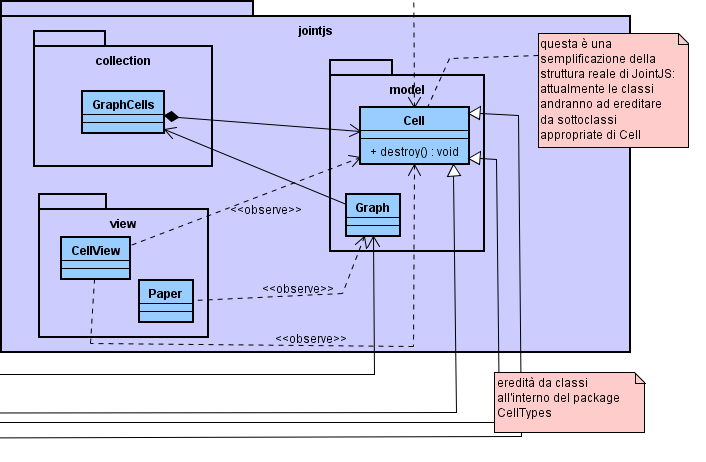
\includegraphics[width=1\textwidth]{img/jointjs.png}}
\caption{Esemplificazione delle classi di \jointjs{}}

\end{figure}

La figura precedente mostra una esemplificazione della gerarchia di classi usata da \proj. Essa mostra tre package distinti, model, view e collection, per indicare che essi derivano da \texttt{Backbone.Model}, \texttt{Backbone.View} e \texttt{Backbone.Collection} rispettivamente.

La creazione di un nuovo diagramma è piuttosto semplice: è sufficiente specificare un \texttt{Graph} sul quale un \texttt{Paper} deve rimanere in ascolto (\emph{observe}). È possibile catturare eventi all'interno del \texttt{Paper} e gestirli di conseguenza.

Il \texttt{Graph} possiede al suo interno una \texttt{GraphCells}. Questa rappresenta il raccoglitore di celle (\texttt{Cell}, che costituiscono gli elementi da cui è composto un \texttt{Graph}. 

Una \texttt{Cell} è osservata da una \texttt{CellView} del tutto simile in funzionamento a quanto descritto in precedenza tra un model ed una view. 

Ereditando da \texttt{Cell} (o meglio, dalle appropriate sottoclassi) possiamo disporre già di svariati metodi già implementati e testati da \jointjs{}.

\section{Architettura di Backbone.js}
%%%%%%%%%%%%%%%%%%%%%%%%%%%%%%%
%%  Architettura di Backbone.js
%%%%%%%%%%%%%%%%%%%%%%%%%%%%%%%



L'appendice che segue è tratta e rielaborata dal libro \emph{Developing Backbone.js Applications}, \emph{Addy Osmani}, \emph{O'Reilly}.

Il pattern seguito dal client di \proj{} ricalca il pattern di \jointjs, basato su \backbonejs. Classificare questo pattern non è un compito semplice: la comunità di Backbone.js è internamente divisa sull'effettiva natura del pattern che implementa. Molti sviluppatori JavaScript non vedono i pattern MVC (Model View Controller) e MVP (Model View Presenter) come mutualmente esclusivi, ma è possibile sviluppare una applicazione che possiede un componente simile al Presenter e considerarla ancora fondata su un tipo di MVC.

Alcuni sviluppatori pensano invece che Backbone.js sia più una implementazione del modello MVP: principalmente il Presenter consiste nella \texttt{Backbone.View}, il modello è rappresentato da \texttt{Backbone.Model} e le view sono rappresentate dai template HTML. 

È possibile rispondere a questa osservazione constatando che \texttt{Backbone.View} è effettivamente capace di assolvere a due compiti, perché essa è flessibile a sufficienza per essere usata per multipli scopi. Questi due compiti sono la View dell'MVC e la Presenter dell'MVP.

Questo porta all'osservazione fatta dall'autore di MarionetteJS, Derick Bailey, il quale afferma che è meglio non forzare Backbone.js a sottostare ad uno specifico design pattern: un design pattern dovrebbe essere una \textbf{guida flessibile} riguardo a come una applicazione potrebbe essere strutturata, e in questo senso Backbone.js non entra né nella definizione di MVC né di MVP.


\section{Pattern creazionali} \label{sec:app_creaz}
%%%%%%%%%%%%%%%%%%%%%%%%%%%%%%
%%  Design pattern creazionali
%%%%%%%%%%%%%%%%%%%%%%%%%%%%%%

\subsection{Dependency injection}

\begin{figure}[H] \label{fig:injector}
	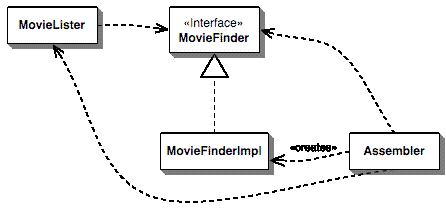
\includegraphics[scale=0.8]{img/injector.png}
	\caption{Dependency Injection.}
\end{figure}

\subsubsection{Scopo} Permette di disaccoppiare il comportamento di una componente dalla risoluzione delle sue dipendenze, semplificando perciò lo sviluppo di un software di grandi dimensioni e allo stesso tempo migliorandone la testabilità.

\subsubsection{Motivazione} Grazie a questo pattern è possibile separare la responsabilità di uso e creazione di un oggetto. Il componente dipendente dovrà solo sapere come usare un servizio richiesto, mentre il compito di creare ed iniettare quest'ultimo spetta ad un injector. Questo permette al componente dipendente di essere altamente configurabile in quanto è fisso solo il suo comportamento.

\subsubsection{Struttura} Sono coinvolti 3 componenti nella dependency injection:
\begin{enumerate}
	\item gli oggetti servizi(ossia un qualsiasi oggetto che potrebbe essere usato);
	\item l'oggetto dipendente da questi servizi;
	\item un injector responsabile di creare ed iniettare i servizi.
\end{enumerate}

\subsubsection{Applicabilità} È possibile applicare il pattern in tre modi differenti:
\begin{itemize}
	\item \textbf{setter injection:} la dipendenza viene iniettata tramite dei metodi setter del component dipendente;
	\item \textbf{costruction injection:} la dipendenza viene iniettata tramite un paramento del costruttore;
	\item \textbf{interface injection:} l'iniezione viene eseguita attraverso l'interfaccia che fornirà un setter a chiunque la implementa.
\end{itemize}

\subsection{Command}

\begin{figure}[H] \label{fig:command}
	
\includegraphics[scale=0.6]{img/command.png}
	\caption{Command.}
\end{figure}

\subsubsection{Scopo} Permette di isolare la porzione di codice che effettua un'azione dal codice che ne richiede l'esecuzione. Tale azione è incapsulata nell'oggetto Command.

\subsubsection{Struttura} Sono coinvolti i seguenti componenti:
\begin{enumerate}
	\item Client: colui che richiede il comando  ed imposta il Receiver;
	\item Invoker: colui che effettua l'invocazione del comando;
	\item Command: interfaccia generica per l'esecuzione del comando;
	\item ConcreteCommand: implementazione del comando che consente di collegare l'invoker con il Receiver;
	\item Receiver: colui che riceve il comando e sa come eseguirlo.
\end{enumerate}

\subsubsection{Applicabilità} È possibile applicare il pattern per:
\begin{itemize}
	\item parametrizzare gli oggetti sull'azione da eseguire;
	\item specificare,accodare ed eseguire richieste molteplici volte;
	\item supportare operazioni di Undo e Redo;
	\item supportare la transazione: un comando equivale ad un'operazione atomica.
\end{itemize}

\subsection{Factory}

\begin{figure}[H] \label{fig:factory}
	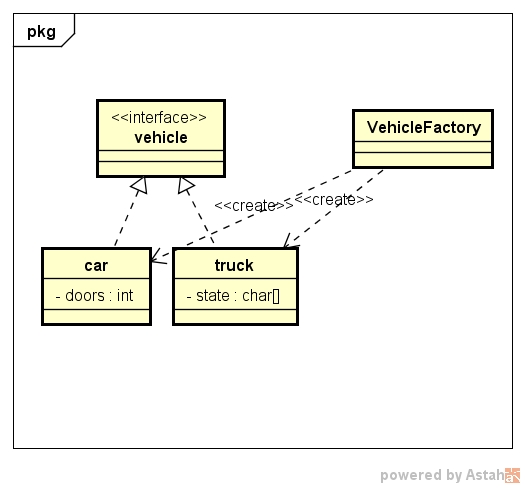
\includegraphics[scale=0.8]{img/factory2.png}
	\caption{Factory.}
\end{figure}

\subsubsection{Scopo} Indirizza il problema della creazione di oggetti senza specificarne la classe esatta fornendo un'interfaccia per creare l'oggetto, ma lascia che le sottoclassidecidano quale oggetto istanziare.

\subsubsection{Struttura} Sono coinvolti i seguenti componenti:
\begin{enumerate}
	\item Creator (VeichleFactory): dichiara la Factory che avrà il compito di ritornare l'oggetto appropriato;
	\item Product (Vehicle): definisce l'interfaccia dell'oggetto che deve essere creato dalla Factory;
	\item ConcreteProduct (Truck,Car): implementa l'oggetto in base ai metodi  definiti dall'interfaccia Product.
\end{enumerate}

\subsubsection{Applicabilità} È possibile applicare il pattern quando:
\begin{itemize}
	\item la creazione di un oggetto preclude il suo riuso senza una duplicazione di codice;
	\item la creazione di un oggetto richide l'accesso ad informazioni o risorse che non dovrebbero essere contenute nella classe di composizione;
	\item la gestione del ciclo di vita degli oggetti gestiti deve essere centralizzata in modo da assicurare un comportamento coerente all'interno dell'applicazione.
\end{itemize}

\subsection{Observer}

\begin{figure}[H] \label{fig:observer}
	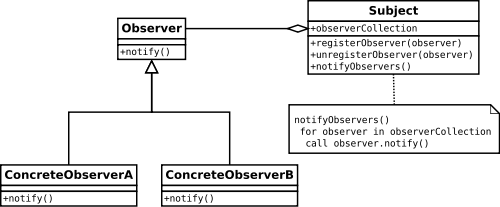
\includegraphics[scale=0.6]{img/observer.png}
	\caption{Observer.}
\end{figure}

\subsubsection{Scopo} Questo pattern viene utilizzato quando si vuole realizzare una dipendenza uno-a-molti in cui il cambiamento di stato di un soggetto venga notiifcato a tutui i soggetti che si sono mostrati interessati.

\subsubsection{Struttura} Sono coinvolti i seguenti componenti:
\begin{enumerate}
	\item Subject: espone l’interfaccia che consente agli osservatori di iscriversi e cancellarsi mantenendi una reference a tutti gli osservatori iscritti;
	\item Observer: espone l’interfaccia che consente di aggiornare gli osservatori in caso di cambio di stato del soggetto osservato;
	\item ConcreteSubject: mantiene lo stato del soggetto osservato e notifica gli osservatori in caso di un cambio di stato;
	\item ConcreteObserver: implementa l’interfaccia dell’Observer definendo il comportamento in caso di cambio di stato del soggetto osservato.
\end{enumerate}

\subsubsection{Applicabilità} È possibile applicare il pattern quando:
\begin{itemize}
	\item in un problema ci sono due aspetti tra loro dipendenti, che possono essere rappresentati come classi che possono essere usati indipendentemente tra loro;
	\item quando il cambiamento di un oggetto provoca un cambiamento in un altro oggetto;
	\item quando un oggetto ha la necessità di comunicare con altri oggetti, senza fare assunzioni sugli altri oggetti.
\end{itemize}


\end{document}
